\documentclass{ieeeaccess}
\usepackage{cite}
\usepackage{amsmath,amssymb,amsfonts}
\usepackage{algorithmic}
\usepackage{algorithm2e}
\usepackage{graphicx}
\usepackage{textcomp}
\usepackage{times}
\usepackage{soul}
\usepackage{url}
\usepackage[hidelinks]{hyperref}
\usepackage[utf8]{inputenc}
\usepackage[small]{caption}
\usepackage{graphicx}
\usepackage{amsmath}
\usepackage{booktabs}
\usepackage{algorithm}
\usepackage{algorithmic}
\usepackage{float} 
\usepackage{subfigure}
\usepackage{xspace}
\usepackage{amsthm}



\urlstyle{same}



\newcommand{\sys}{Combo\xspace}
\newcommand{\eg}{e.g.,\xspace}
\newcommand{\ie}{i.e.,\xspace}


\newenvironment{packeditemize}{\begin{list}{$\bullet$}{\setlength{\itemsep}{0.5pt}\addtolength{\labelwidth}{-4pt}\setlength{\leftmargin}{\labelwidth}\setlength{\listparindent}{\parindent}\setlength{\parsep}{1pt}\setlength{\topsep}{0pt}}}{\end{list}}



\def\BibTeX{{\rm B\kern-.05em{\sc i\kern-.025em b}\kern-.08em
    T\kern-.1667em\lower.7ex\hbox{E}\kern-.125emX}}
\begin{document}
\history{Date of publication xxxx 00, 0000, date of current version xxxx 00, 0000.}
\doi{10.1109/ACCESS.2017.DOI}



\title{Bandwidth-Aware Decentralized Federated Learning}
\author{\uppercase{Jingyan Jiang}\authorrefmark{1},
\uppercase{Chenghao Hu\authorrefmark{2}, Zhi Wang\authorrefmark{3} and Liang Hu}.\authorrefmark{4}}
\address[1]{College of Computer Science and Technology, Jilin University (e-mail: jiangjy14@mails.jlu.edu.cn)}
\address[2]{Graduate School at Shenzhen, Tsinghua University (huch16@mails.tsinghua.edu.cn)}
\address[3]{Graduate School at Shenzhen, Tsinghua University (wangzhi@sz.tsinghua.edu.cn)}
\address[4]{College of Computer Science and Technology, Jilin University (hul@jlu.edu.cn)}

% \tfootnote{This paragraph of the first footnote will contain support 
% information, including sponsor and financial support acknowledgment. For 
% example, ``This work was supported in part by the U.S. Department of 
% Commerce under Grant BS123456.''}

\markboth
{Author \headeretal: Preparation of Papers for IEEE TRANSACTIONS and JOURNALS}
{Author \headeretal: Preparation of Papers for IEEE TRANSACTIONS and JOURNALS}

\corresp{Corresponding author: First A. Author (e-mail: author@ boulder.nist.gov).}

\begin{abstract}
The emerging concern about data privacy and security has motivated the proposal of \emph{federated learning}, which allows nodes to only synchronize the locally-trained models instead their own original data. Conventional federated learning architecture, inherited from the parameter server design, relies on highly centralized topologies and the assumption of large nodes-to-server bandwidths. However, in real-world federated learning scenarios the network capacities between nodes are highly uniformly distributed and smaller than that in a datacenter. It is of great challenges for conventional federated learning approaches to efficiently utilize network capacities between nodes. In this paper, we propose a model segment level decentralized federated learning to tackle this problem. In particular, we propose a segmented gossip approach, which not only makes full utilization of node-to-node bandwidth, but also has good training convergence. The experimental results show that even the training time can be highly reduced as compared to centralized federated learning.
\end{abstract}

\begin{keywords}
Enter key words or phrases in alphabetical 
order, separated by commas. For a list of suggested keywords, send a blank 
e-mail to keywords@ieee.org or visit \underline
{http://www.ieee.org/organizations/pubs/ani\_prod/keywrd98.txt}
\end{keywords}

\titlepgskip=-15pt

\maketitle
\section{Introduction}

% Data privacy Federated Learning proposed,

Recent years have witnessed a rapid growth of deep learning algorithms which achieve and even transcend the human-level accuracy on nature language processing and computer vision \cite{devlin2018bert:,he2016deep}, thanks to the massive amount of data collected. To improve the deep learning performance, it is of great demand for different entities to contribute their own data and train models together. In such collaborative training, the concern about data leakage has motivated \emph{federated learning} \cite{McMahan2017FL}, which allows nodes to only synchronize the locally-trained models instead of their own original data. 

A general federated learning system uses a central parameter server to coordinate the large federation of the participating workers (workers and nodes are used interchangeably in this paper). The workers train a local model with their own dataset and send the model updates (\eg gradients or parameters) periodically to a centralized server for synchronization. To reduce the risk of single point failure, a couple of decentralized synchronization methods have been proposed. All-reduce \cite{patarasuk2009allreduce} adopts an all-to-all scheme, i.e., each worker sends the local model updates to all other workers. It achieves the same synchronization effect as parameter server but consumes much bandwidth resource between works. When the model updates from all nodes in the system are sent to all other nodes, the performance is highly degraded. To reduce the transmission cost, gossip based model synchronization \cite{daily2018gossipgrad:,haas2002gossip-based} is proposed: workers send local updates to only one or a group of selected nodes.

In real-world federated learning scenarios, the network capacities between nodes are highly uniformly distributed and smaller than that in a datacenter \cite{vulimiri2015global}. Thus, it is still extremely bandwidth costly when workers send the \emph{full} model updates (e.g., the size can be up to $1360$MB in $BERT_{LARGE}$ \cite{devlin2018bert:}). An intuitive question is then, is it possible for workers to synchronize the model \emph{partially}, from/to \emph{only} a part of the workers, and still achieve good training results? 

Our answer to this question is a novel decentralized federated learning design, introducing a segmented gossip approach, which not only makes full utilization of node-to-node bandwidth by transmitting model \emph{segmentations} in a peer-to-peer manner, but also has good training convergence by carefully forming dynamical synchronization gossiping groups. In particular, the details of the design and the contributions are summarized as follows.

First, we propose a model segmentation level synchronization mechanism. We ``split'' a model into a set of segmentations---subsets which contain the same number of model parameters that are not overlapped with each other. Workers perform segmentation level update by aggregating a local segmentation with the corresponding segmentation from $k$ other workers. Based on our analysis, $k$ can be much smaller than the number of all workers, to achieve good convergence for the training process. 

%Second, we a propose bandwidth-aware gossiping strategy, to dynamically select the $k$ neighbors for each training iteration. Our objective is to maximize the utilization of bandwidth capacities between workers, which are different for different \emph{paths} between worker pairs and dynamically changing overtime. Our gossiping algorithm monitors and predicts the path capacity, and forms worker neighborhood in a path capacity ``saturation'' manner that marginally let pairs of workers with spare bandwidth become gossip neighbors.

Second, we propose a decentralized federated learning design, borrow the idea from gossip protocol; each worker stochastically selects a few workers to transfer the model segment for each training iteration. Our objective is to maximize the utilization of bandwidth capacities between workers and split the bill of communication cost. To improve the convergence performance of our solution, we introduce ``Model Replica'' to guarantee the enough information from different workers. The theory analysis proves that our solution has well convergence property.

Third, we implement the model segmentation strategy and the gossiping strategy into a prototype called \sys, and design experiments to evaluate its performance. Our results show that our design significantly reduces the training time in practical network topology and bandwidth setup, with only slightly accuracy degrade. 


%  We simulate both the training and transferring process to evaluate the design of \sys. The simulation results show that \sys (1)significantly reduces communication time, by *** compares to *** (2)still maintains the training accuracy compares to the state-of-art method, (3)high scalability: 2X more workers, ** speed up in time.


% In summary, the main contributions of this work can be listed as follows:
% \begin{packeditemize}
%     \item We proposed a new decentralized synchronization scheme which adopts the segmented transmission to fully exploit the bandwidth of a single worker.
%     \item We designed a new federated learning system, \sys
%     \item We simulated the \sys learning process.
% \end{packeditemize}
%

\section{Background and }


\begin{algorithm}[!t]

\caption{Rounding-based Approximation Algorithm - RA}

\renewcommand{\algorithmicrequire}{\textbf{Input:}}
\renewcommand{\algorithmicensure}{\textbf{Output:}}

\begin{algorithmic}[1]
\REQUIRE $S, Q, I, J, H, \Delta t,\{Y^q\}_{\forall q}, \{A^q\}_{\forall q},\{S^q_{ij}(h)\}_{\forall q,i,j,h},$\\
$\{B_{is}\}_{i,s}, \{V_i(h)\}_{\forall i,h}, \{c_i\}_{\forall i}$
\ENSURE $\{\bar{x}_{is}(h)\}_{\forall i,s,h}$, $\{\bar{y}_{ijs}^q(h)\}_{\forall q,i,j,s,h}$

\STATE Solve the relaxed LP (8) using interior point method.
\STATE Obtain the optimal fraction solution $\{\hat{x}_{is}(h)\}$ and $\{\hat{y}_{ijs}^q(h)\}$
\FOR {$i \in [I]$, $j\in[J]$, $h \in H$}
	\STATE $\Omega \leftarrow \{\hat{y}^q_{ijs}(h), \forall q\in [Q], s \in [S]| \hat{x}_{is}(h) \text{ is fractional}\}$
	\STATE $\Theta, \Theta_{all}, \{z^q_{ijs}(h)\} \leftarrow $SC($Q, \Omega$)
	\FOR {$q \in \{q \in [Q]|\Theta^q \in \Theta_{all} \}$}
		\STATE Select the first $s$ in $\Theta$ that exists in $\Theta^q$ as $\hat{s}$
		\FOR {$s \in \Theta^q \setminus {\hat{s}}$}
		    \IF {$z^q_{ij\hat{s}}(h) - \lfloor z^q_{ij\hat{s}}(h)\rfloor \leq \lceil z^q_{ij{s}}(h)\rceil -z^q_{ij{s}}(h)$}
		        \STATE $z^q_{ij\hat{s}}(h) \leftarrow z^q_{ij\hat{s}}(h) + z^q_{ij{s}}(h) -\lfloor z^q_{ij{s}}(h)\rfloor$
		        \STATE $z^q_{ij{s}}(h) \leftarrow \lfloor z^q_{ij{s}}(h)\rfloor$
		    \ELSE
		        \STATE $z^q_{ij\hat{s}}(h) \leftarrow z^q_{ij\hat{s}}(h) - (\lceil z^q_{ij{s}}(h)\rceil -z^q_{ij{s}}(h))$
		        \STATE $z^q_{ij{s}}(h) \leftarrow \lceil z^q_{ij{s}}(h)\rceil$
		    \ENDIF
% 			\STATE $\gamma_1 \leftarrow z^q_{ij{s}}(h) - \lfloor z^q_{ij{s}}(h)\rfloor; \gamma_2 \leftarrow \lceil z^q_{ij{s}}(h)\rceil -  z^q_{ij{s}}(h)$
% 			\STATE With probability $\frac{\gamma_2}{\gamma_1 + \gamma_2}$ set 
% 				$$z^q_{ij{s}}(h) \leftarrow z^q_{ij{s}}(h) - \gamma_1; z^q_{ij\hat{s}}(h)\leftarrow z^q_{ij\hat{s}}(h) + \gamma_1$$
% 			\STATE With probability $\frac{\gamma_1}{\gamma_1 + \gamma_2}$ set
% 				$$z^q_{ij{s}}(h) \leftarrow z^q_{ij{s}}(h) + \gamma_2; z^q_{ij\hat{s}}(h)\leftarrow z^q_{ij\hat{s}}(h) - \gamma_2$$
		\ENDFOR
	\ENDFOR
	\FOR {$s\in[S]$}
		\IF {$\hat{x}_{is}(h)$ is fractional}
			\STATE $\bar{x}_{is}(h) \leftarrow \lceil\sum\limits_{q\in[Q]}\sum\limits_{j\in[J]}z^q_{ij{s}}(h)\rceil$
		\ELSE
			\STATE $\bar{x}_{is}(h) \leftarrow \hat{x}_{is}(h)$
		\ENDIF
	\ENDFOR
\ENDFOR
\STATE Fix the variable $\{{x}_{is}(h)\}$ in (8) to $\{\bar{x}_{is}(h)\}$ and solve the new LP (8) again to obtain $\{\bar{y}_{ijs}^q(h)\}$

\end{algorithmic}	\label{RA} 
\end{algorithm}
\section{Related work}
\textbf{Distributed ML}
Conventional distributed machine learning systems are centralized, workers periodically send the local updates to a (a set of) parameter servers (PS), such as SparkNet\cite{moritz2016sparknet:}, Tensorflow\cite{abadi2016tensorflow:} and traditional federated learning systems \cite{konecny2015federated,konevcny2016federated}. To avoid bottleneck and single point failure, \cite{li2014scaling,mlsys2019towards} aim to scale PS for  better network utilization. Although these scaling methods could increase the accumulative bandwidth at the server side, they are still suffering the long convergence time when the network is poor.
\begin{algorithm}[!t]

\caption{Federated Averaging (FedAvg)}

\renewcommand{\algorithmicrequire}{\textbf{Input:}}
\renewcommand{\algorithmicensure}{\textbf{Output:}}

\begin{algorithmic}[1]
\SetKwFunction{FC}{{ClientUpdatae}}
\REQUIRE $K, T, \eta, E, w_0, N, n, n_k, p_k,  k = 1,...,N $

\STATE \textbf{Server executes:}
\FOR {$t = 0, ...,T-1$}
    \STATE server selects a subset $S_t$ of K workers at random (each worker $k$ is chosen with probability $p_k$)
    \STATE send $w_t$ to all chosen workers
    \FOR{each client $k \in S_t$ in parallel}
        \STATE $w^k_{t+1} \leftarrow$\FC{$k,w_{t}$}
    \ENDFOR
    \STATE $w_{t+1} \leftarrow \sum ^{K}_{k=1} \frac{n_k}{n}w^k_{t+1}$
\ENDFOR

\item[]

\STATE \FC{$k,w_{t}$}//Run on worker $k$
    {\STATE \quad worker $k$ updates $w_t$ for $E$ epoches of SGD on $F_k$ \\ \quad with step size $\eta$ to obtain $w_{t+1}$
\RETURN $w_{t+1}$ }


\end{algorithmic}	\label{Fedavg} 
\end{algorithm}


An alternative solution is decentralized architecture, the workers exchange updates directly using all-reduce scheme, with a communication cost $O(n^2)$ for $n$ workers. To reduce the huge communication costs, an intuitive approach is to take the advantage of topology. Baidu first introduced Ring-allreduce \cite{allreduce}, which is a bandwidth-optimal way to do an allreduce. The workers involved are arranged in a ring, each worker send gradients to the next clockwise worker and receives from the previous one. In this way, it reduces the communication complexity to linear growth in scale. similarly, the tree \cite{li2015malt:} and graph \cite{agarwal2014a} topologies are proposed to reduce the communication cost. However, these approaches may need multiple hops between workers, resulting in slow convergence. Instead of topology-based method, Ako \cite{watcharapichat2016ako:} propose a partial gradient updates method. In each synchronization round, each worker sends a gradient partition to every other worker. Obviously, Ako reduces the synchronization time and the communication overhead depends on the partition size and the worker number. 
 
Although these existing approaches perform well in distributed ML, they aggregate gradients every epoch, which still face heavy communication cost and is not practical in federated learning with slow internet connections. 

 
% However, in the federated learning scenario, it is still a huge cost to communicate with every other worker.
%To reduce the huge communication costs in decentralized architecture and speed up the training time, 

\textbf{Communication efficient FL} 
A main research focus of federated learning is to reduce the communication cost. \cite{konevcny2016federated} propose structured updates and sketched updates to reduce the exchange data size at the cost of accuracy loss. \cite{McMahan2017FL} propose the federated averaging algorithm (FedAvg) to reduce the parameter updates significantly. FedAvg aggregates parameters after several epochs. In each synchronization round, it selects a fraction of workers and computes the gradient of the loss over all the data held by these workers. These methods are based on the PS architecture, which face the network congestion when the updates arrive at the PS concurrently.  

%\cite{konecny2015federated,konevcny2016federated,McMahan2017FL,mcmahan2018learning}, to reduced the upload communication, \cite{konevcny2016federated} proposed structured updates and sketched updates %\cite{konecný2015federated,McMahan2017FL,mcmahan2018learning,mlsys2019towards,konevcny2016federated} is focus on  

\textbf{Gossip protocol in ML}
The gossip protocol widely used in distributed systems \cite{baraglia2013a,haas2002gossip-based}, each worker sends out message to a set of other workers, the message propagates through the whole network worker by worker. \cite{blot2016gossip} first introduced the gossip protocol in deep learning. They propose GoSGD, using sum-weight gossip protocol to share the updates with selective workers. The results show good consensus convergence properties. \cite{daily2018gossipgrad:} propose GossipGraD, which is a gossip based SGD algorithm for large scale deep learning system and reduces the communication complexity to $O(1)$. 

However, in federated learning, network connections between geo-distributed workers usually could not be fully utilized because of the bottleneck, which are ignored in these approaches. 
%In this work, we bring the Gossip protocol to federated learning, which maximizes the utilization of bandwidth capacities between workers and transfer the smaller parameter segments to reduce the communication cost and speed up convergence.

%these works did not consider the network connection between geo-distributed workers 
%
%federated learning
%
%While, to bring the Gossip protocol to federated learning is still an open issue. 

%These approaches did not consider the partial updates and still suffer from the slow convergence in federated learning scenario.

%which is a new way to share information between different threads inspired by gossip algorithms and showing good consensus con- vergence properties. 
%(1)Conventional gossip protocol \cite{blot2016gossip} (2)Distributed machine learning with gossip \cite{blot2016gossip} \cite{daily2018gossipgrad:}



\section{Bandwidth-Aware Segmented Gossip Aggregation}

Now consider the network topology with $n$ workers. An all-reduce worker pushes $n-1$ local model replicates to the other workers through $n-1$ links while a gossip worker is expected to push one local model replicate out through only one link. Within a datacenter where the workers are connected by the local area network, they can always communicate with each other at maximum bandwidth thus the gossip worker can achieve great speed up as the transmission size is drastically reduced.

However, in the federated learning context where the workers are geo-distributed, the real bandwidth between the workers is typically small due to the potential bottleneck of WAN. Thus the traditional gossip-based schemes can not make full use of the worker's bandwidth because the transmissions are limited in one or few links. We propose the \emph{Segmented Gossip Aggregation} to solve this problem by "splitting" the transmission task and feeding them into more links.

%In the \sys solution, the worker takes the responsibility of data flow: to communicate actively the local model with a portion of peers, transfer local model and aggregate local model. The intuition of \textit{Active} borrows the idea from Gossip-based protocols in which the workers actively push the models to peers. By doing this, the heavy traffic in $n$ links of parameter server could be dissolved among the $n(n-1)$ links between $n$ workers.
%

\subsubsection{Segmented Pulling}

Fig. \ref{Fig: Segment sub.1} illustrates the transfer procedure with segmented gossip aggregation which we name it \emph{segmented pulling.} In the aggregation phase, the worker needs to receive the model parameters from others. While the naive gossip-based synchronization schemes require the worker to collect the whole model parameters, segmented pulling allows the worker to pull different parts of the model parameters from different workers and rebuild a mixed model for aggregation.

Let $\mathcal{W}$ denote the model parameters. The worker firstly breaks the structure of $\mathcal{W}$ into $S$ segments without overlapping such that
\begin{equation}
    \mathcal{W} = (\mathcal{W}[1],\mathcal{W}[2],\dots,\mathcal{W}[S])
\end{equation}

For each segment $l$, the worker chooses a peer worker which we denote it as $j_l$ and then actively pulls the corresponding segment $\mathcal{W}_{j_l}[l]$ from it. Note that this step is parallelized to make full use of the bandwidth. When the worker fetches all the model segments back, a new mixed model $\mathcal{W}^\prime$ can be rebuilt from the segments such that
\begin{equation}
    \mathcal{W}^\prime = (\mathcal{W}_{j_1}[1],\mathcal{W}_{j_2}[2],\dots,\mathcal{W}_{j_l}[S])
\end{equation}

The naive gossip-based scheme pulls all the segments from a single peer worker. However, with segmented pulling, if we choose a different peer for each segment, the total transmission size is still equal to one model, like the naive gossip-based schemes, but the traffic is dissolved among not one but $S$ links.


\subsubsection{Bandwidth-Aware Worker Selection}
The WAN bandwidth not only varies significantly between different regions (e.g., up to $12 \times$ of bandwidth variance between geographically-close regions and distant regions), but also is time-varying (e.g., up to $10 \times$ of bandwidth variance within a day), as shown by other systems \ref{}.  Thus, to reduce the transmission time, we tend to select 

Taking the advantage of epsilon-greedy, we 


%\begin{figure}[H]
%\centering 
%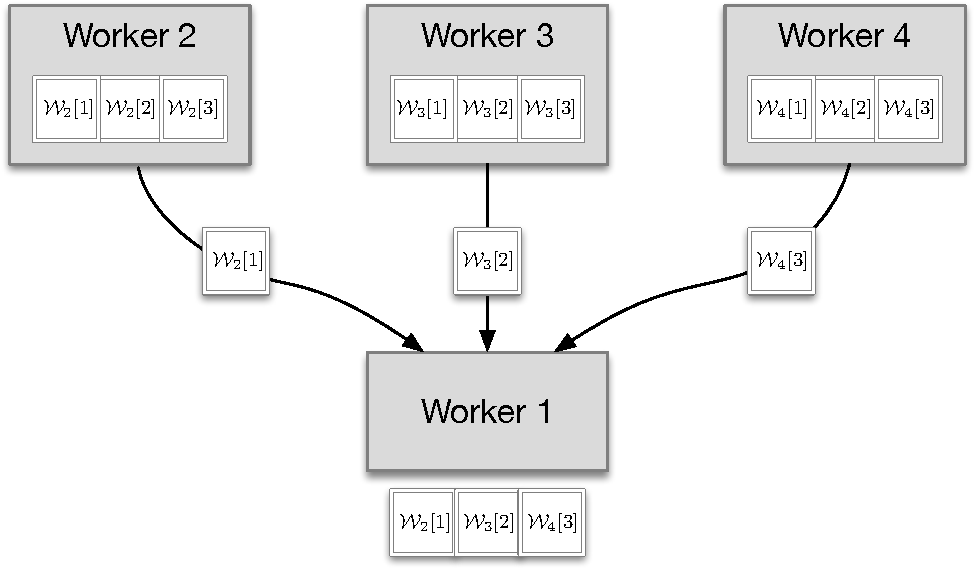
\includegraphics[width=0.3\textwidth]{pics/seg_pull.pdf}
%\caption{Segmented Pulling}
%\label{Fig: seg-pull}
%\end{figure}


\subsubsection{Model Replica}

% Like other gossip-based approaches, we use random partial aggregation as an approximation of the global aggregation. But if the number of the participating workers is too big, which could be common in a federated learning context, there might be huge deviation in such approximation if the worker aggregates local model with only one external model as there are many of them. 
% 

In traditional distributed ML scenario within the datacenter, the gossip-based solutions can choose only one other worker for aggregation but still achieve excellent convergence, because the workers ``gossip" with each other frequently such that the update of each worker are propagated through the whole network before they become too stale\cite{daily2018gossipgrad:}. However, for communication efficient FL systems, the staleness of the model updates is hard to bound as the models are trained separately for up to a few epochs. 
 

Thus as a compromise, we set a hyper-parameter \textit{Model Replica} $R$ which represents the number of the mixed model gathered by segmented pulling. To rebuild $R$ mixed models, the worker will pull $S \times R$ segments from peers. Thus increasing the value of $R$ means more segments have to be transferred through the network, which may cause bandwidth overhead. But this is necessary to accelerate the propagation and ensure the model quality. Since there is no centralized server bottleneck, the model training speed could still be faster even with extra transmission.


\subsubsection{Bandwidth-Aware Gossip Aggregation}
\begin{algorithm}[!t]

\caption{Bandwidth-Aware Combo (BACombo)}

\renewcommand{\algorithmicrequire}{\textbf{Input:}}
\renewcommand{\algorithmicensure}{\textbf{Output:}}
\SetKwFunction{SP}{{SegPulling}}
\SetKwFunction{SA}{{SegAggregation}}


\begin{algorithmic}[1]
\REQUIRE $K, T, \eta, E, \widetilde{w}_0, N, S, \epsilon $

\STATE \textbf{Each worker $i$ executes:}
\STATE $ B \leftarrow \mathbf{0} $

\FOR {$t = 0, ...,T-1$}
    \STATE $r_t \leftarrow Random()$ 
    \STATE updates ${ w}_{t}$ for $E$ epoches of SGD on $F_i$  with step size $\eta$ to obtain ${ w}_{t+1}$
    \IF{ $r_t < \epsilon $}{
        \STATE %$ \{{w}_{t,k}^\prime\}, J, \{D_j\} \leftarrow $ 
        \SP{$Random(),K, N,i$}
        \STATE update $B$ based on the \textbf{BandwidthPrediction}$(J)$}
    \ELSE {
        \STATE %$ \{{w}_{t,k}^\prime\}, J, \{D_j\} \leftarrow $ 
        \SP{$Greedy(),K, N,i$}
    } 
    \ENDIF
    \STATE $\widetilde{{w}}_{t+1} \leftarrow$ \textbf{SegAggregation} $(\{{w}_{t,k}^\prime\},{{w}}_{t+1},J ,\{D_j\})$
\ENDFOR
\item[]

\STATE \SP{$k,w_{t}$}//Run on worker $k$
{
    \STATE \quad worker $k$ updates $w_t$ for $E$ epoches of SGD on $F_k$ \\ \quad with step size $\eta$ to obtain $w_{t+1}$
\RETURN $w_{t+1}$ 
}

\item[]

\STATE \SA{$k,w_{t}$}//Run on worker $k$
{
    \STATE \quad worker $k$ updates $w_t$ for $E$ epoches of SGD on $F_k$ \\ \quad with step size $\eta$ to obtain $w_{t+1}$
\RETURN $w_{t+1}$ 
}

\end{algorithmic}	\label{BACombo} 
\end{algorithm}

            % \STATE worker selects a subset $S_{t}$ of S segments at random (each segments $s$ is chosen from  with probability $p_s$)
            
        %             \FOR {$ k = 1, ..., K$}
            
        % \ENDFOR
                % \STATE worker selects a subset $S_{t, s, r}$ of  workers at random (each worker $k$ is chosen with probability $p_k$)
%The \sys worker updates its local model using multiple "local models" from peers, each local model is a composition of model segments from different peers, we call the composition \textit{Model Replica}.

%
%the workers pull their local model to peers instead of center server.  
%
%When a worker $i$ finishes the local training and seeking to do the model aggregation, it reports its status to the index server. And then the server randomly samples a subset $K_i$ from all the participating workers as the aggregation candidates of worker $i$ and send the information about $K_i$ to worker $i$. To control the training progress, the workers of $K_i$ should have the same training iterations. When worker $i$ receives the candidate list $K_i$, it proactively fetches the model from the candidate workers, do the aggregation and then continue training on the local dataset. We use an index server to track the information of workers instead of storing peer information on the workers directly because with the growth of the workers and the variation of the network environment, the synchronization overhead can be very huge.
%
% By increasing the initiative of the workers, the bottleneck of server is removed because the communication of the server is trivial and the model parameters, which is the heavy part, are transferred among $n(n-1)$ links of all the workers.

%\subsection{Worker Segmented Transfer and Aggregation}
%After ... , the worker will ... transfer and aggregation...
% 一句话描述他们要干什么


%The idea of pulling model parameters from peers is quite similar with the Gossip-based protocols in which the workers randomly push the models to others. So they are facing the same challenge that the overall transmission quantity is increased for a single worker. In the traditional parameter server architecture, in one global iteration, the worker only has to send and receive for one time. But with the gossip methods, each worker is expected to send and receive for $|K_i|$ times in one iteration. 

%
%As shows in Figure \ref{Fig: Segment sub.1}, when the worker $i$ receives the manifest of $K_i$ candidate worker list from index server.  if the model are break in to $S$ and the replica is set to be $R$. For each segment $l$, worker $i$ selectively choose a worker $N_l$ from the candidate list, and then fetch the corresponding segment from worker $N_l$ which we denote as $\mathcal{W}[l;N_l]$. Note that this step can be parallelized, and to simplify, we use a uniform random sampling method to choose the peers. 

%With the segmented transfer method, worker $i$ receives model information from multiple peers with the transfer size equal to one model. Thus in the aggregation phase, the aggregation result can be affected by more datasets and this could help to increase the generality of the model. But if the number of the participating workers is too big, which could be common in a federated learning context, the segments can only cover few workers. Increasing the number of segments might help but an extremely small segment size could lead to over-mottled parameters. Thus as a compromise, we set a hyper-parameter $R(eplica)$ which means the number of the mixed model rebuilt by Segmented Transfer. 
%
%Another shining point of segmented transfer is privacy preserving. The complete model parameter or gradient set has the potential to leak private data information under attack. Instead of pulling the whole model from peers, \sys only collects a random subset of the parameters, which helps to preserve the data privacy. 

\begin{figure}[H]
\centering 
\subfigure[Segmented Pulling]{
\label{Fig: Segment sub.1}
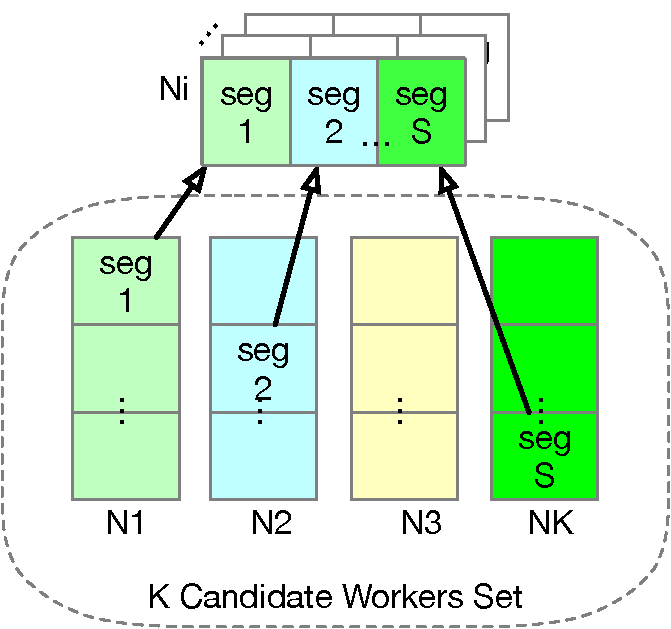
\includegraphics[width=0.2\textwidth]{pics/transfer.pdf}}
\subfigure[Segmented Aggregation]{
\label{Fig: Segment sub.2}
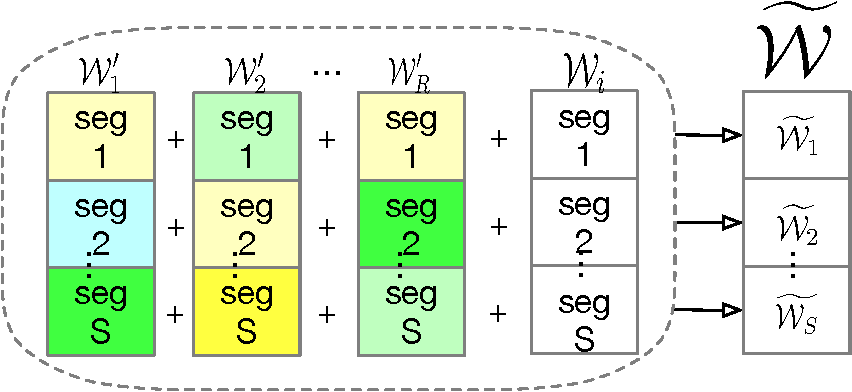
\includegraphics[width=0.225\textwidth]{pics/aggregation.pdf}}
\caption{Segmented Gossip Aggregation}
\label{Fig: Segmented schema}
\end{figure}

\subsubsection{Segmented Aggregation}
%When it fetches all the segments back, a new mixed model can be rebuilt as:
%\begin{equation}
%    \mathcal{W}^\prime = \bigcup_{l = 1}^{S} \mathcal{W}[l;N_l] \label{eq:seg_union}
%\end{equation}
Typically the model aggregation uses weighted averaging of the received model parameters with the worker's dataset size as weight. But in segmented gossip aggregation, the mixed models are patched together from different workers, so it is hard to set a reasonable weight for the mixed model as a whole. For such case, we use a segment-wise model aggregation. 

 Assume the worker $i$ has fetched all the segments and rebuilt $R$ mixed models which we represent as $\mathcal{W}^\prime_1,\mathcal{W}^\prime_2, \dots ,\mathcal{W}^\prime_R$. Then for each segment $l$, we have $R$ mixed models and one local model to aggregate. Let $P_l$ denote the set of the workers which provide the segment $l$ (worker $i$ itself is contained too) and $|D_j|$ denote the dataset size of worker $j$, then we can aggregate segment $l$ by:
 
 \begin{equation}
 \label{eq:seg_agg}
     \widetilde{\mathcal{W}}[l] = \frac{\sum_{j\in P_l}|D_j|\mathcal{W}_j[l]}{\sum_{j\in P_l}|D_j|}
 \end{equation}

Combine all the aggregated segments, and we can rebuild the final aggregation result by 
\begin{equation}
    \mathcal{W} = (\widetilde{\mathcal{W}}[1],\widetilde{\mathcal{W}}[2],\dots,\widetilde{\mathcal{W}}[S])
\end{equation}
And then the worker can continue its training until next aggregation phase comes.
 

\section{\sys Design}
In this section, we introduce \sys, a decentralized federated learning system based on segmented gossip aggregation. We firstly present the implementation details of \sys, then discuss how it handles the dynamic nature of FL workers, and finally, we give a brief analysis of the convergence of \sys.

\subsection{Implementation Details}
As a decentralized FL system, we focus on the design of the workers as the participation of the centralized server is not required during the training. However, it's important to notice that before the training starts, the server has to initialize the model parameters of each worker with the same value otherwise the training may fail to converge. 

A \sys worker follows a stateful training process as illustrated by the numbered steps in Fig.\ref{Fig: worker-arch}. At each iteration, the workers (1) update the model with local dataset and meanwhile, (2) send the segment pulling requests to other workers, once the update is finished, they (3) send the segments to the requestors as a response of the pulling requests and when all the pulling requests are satisfied, the workers (4) aggregate the model segments and start next iteration. Next, we describe the implementation details of these steps.

\noindent{\bf (1) Local Update.} The learning process starts with the worker updating the model with the local dataset. The worker takes the aggregation result of the last iteration as the input model and updates it using stochastic gradient descent(SGD) with the local data. To reduce the communication cost, the local update may contain multiple SGD rounds before the communication with other workers. We denote the communication interval or the number of SGD rounds as $\tau$, which, in typical FL systems, could be up to a few epochs.

\noindent{\bf (2) Segments Pulling.} The workers firstly decide how to partition the model. They don't have to follow the same partition rule, but for simplicity, we assume they partition the model into $S$ segments in the same way. For each segment, the worker has to select $R$ peers and sends the \emph{pulling request}, which contains a segment description and a unique identifier of the worker to indicate which part of the model is to be sent and whom it suppose to be sent to. 

Each worker has to send $S\times R$ segment pulling requests to the other workers, and \sys tries to distribute these requests evenly among all the workers to engage more links and balance the transmission workload. Thus for each request, the target worker is randomly selected from all the other workers without replacement until there is no option left, which means when $S\times R \leq n$, all the segments come from different workers. Note that for each iteration, the pulling requests can be sent even before the local update starts; in this way, the target workers can send the segments immediately when the local model is ready.

\noindent{\bf (3) Segments Sending.} The sending procedure is a twin action of the segments pulling. When the worker finishes the local update, it is ready to send its update result to others. Rather than actively pushing the model, the worker only dispatches the model segments according to the received pulling requests.

\noindent{\bf (4) Model Aggregation.} While the worker is providing the model segments to others, it is also receiving the segments it has requested previously. The model aggregation phase is blocked until all the pulling requests are satisfied, then the worker aggregates the external model segments with the local model using \eqref{eq:seg_agg} and put the aggregated segments together to rebuild the model. With the aggregation result, the worker gets back to the first step and starts the next training iteration.


\begin{figure}[H]
\centering 
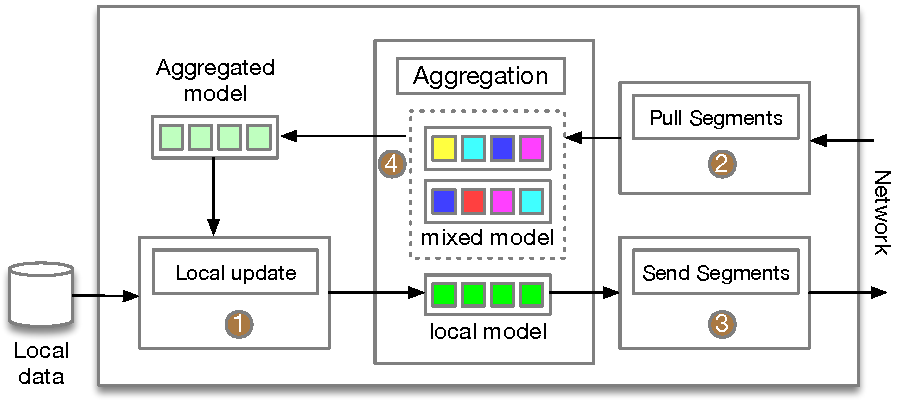
\includegraphics[width=0.49\textwidth]{pics/worker_arch.pdf}
\caption{The architecture of \sys workers}
\label{Fig: worker-arch}
\end{figure}



\subsection{Dynamic Workers}
In the context of federated learning, the participating workers are more likely to be mobile phones and embedded devices, which are often not connected to a power supply and stable network. Thus the workers in FL system are highly dynamic and unstable, and they can join and exit the federation at any time. 

Traditional distributed systems adopt the heartbeat packet and time threshold to check the status of the workers. However, these methods are not applicable with the FL system for the next two reasons: 1) The server has to maintain the heartbeat connection with all the participating workers which limits the scalability of the system. 2) The computation times of each worker vary significantly due to the difference in the computing devices and network environment.

Fortunately, the design of \sys allows us to solve this problem decently. If the worker exits accidentally, the pulling requests it sends to other workers can be canceled immediately when the target workers find it unreachable. For those workers who have requested segments from the offline worker, they can monitor the status of the target workers, and once they see the connection with the target worker is lost, they can mark it as offline, resend the request to another worker and stop pulling from the offline worker. If it is a false report due to the network fluctuation or the offline worker comes back, the offline flag can be removed as long as the communication is reestablished. 

The participation of a new worker is relatively easy to handle. When a new worker comes to the federation, it first requests a worker list either from a server or an old worker. Then it pulls the segments and aggregates them as normal only without its own local model. With the aggregation result, it can start the training with its local dataset. When it sends the pulling requests to the target workers, the target worker adds the newcomer to the worker list. Since the new worker sends the pull requests to many workers in a single iteration, its existence will be quickly noticed by all other workers, and then the new worker successfully joins the federation.




\subsection{Convergence Analysis}

\newtheorem{theorem}{\bf Theorem}
\newtheorem{define}{\bf Definition}
\newtheorem{assumption}{\bf Assumption}

Generally, the deep learning uses the gradient descent algorithms to find the model parameters that minimize a user-defined loss function which we denote it as $F(\mathcal{W})$. For the loss function, we make the following assumptions.

\begin{assumption}
{\bf (Loss function)} $F(\mathcal{W})$ is a convex function with bounded second derivative such that
\begin{equation}
    \mu \leq ||\nabla^2F(\mathcal{W})|| \leq L
\end{equation}
\end{assumption}

In a centralized learning system, the model parameters are updated with the gradient $\nabla F(\mathcal{W})$ calculated from the whole dataset. But with the federated settings, the worker $i$ updates the model with the gradient of a subset of data and we denote it as $\nabla F_i(\mathcal{W})$. To capture the divergence of these two gradients, we make the next definition.

\begin{define}
    {\bf (Gradient Divergence)} For any worker $i$ and model parameter $\mathcal{W}$, We define $\delta$ as the upper bound of the divergence between local and global gradients.
    \begin{equation}
      || \nabla F_i(\mathcal{W}) - \nabla F(\mathcal{W})|| \leq \delta
    \end{equation}
\end{define}

For a worker $i$ in our proposed system, at iteration $t$, the local model parameter $\mathcal{W}_{t,i}$ is an aggregation result of the local model and a few mixed models rebuilt from segments. As a contrast, we denote $\mathcal{W}_{t}$ as the aggregation result of all the nodes, which is the output of $FedAvg$ algorithm. Like the gradient divergence, we define aggregation divergence to measure the aggregation result.

\begin{define}
    {\bf (Aggregation Divergence)} For any worker $i$ at iteration $t$, we define $\rho$ as the upper bound of the divergence between partial and global aggregation.
    \begin{equation}
      || \mathcal{W}_{t,i} - \mathcal{W}_{t}|| \leq \rho
    \end{equation}
\end{define}

With the above assumption and definitions, we can present the convergence result of \sys. 

\begin{theorem}
\label{trm:converge}
    Let $\mathcal{W}^*$ denote the global optimum and $\mathcal{W}_0$ denote the initial model parameters, worker $i$ performs gradient descent on local dataset for $\tau$ times with learning rate $\alpha \leq \frac{1}{L}$ and then pull the segments to aggregate, the aggregation result is $\mathcal{W}_{t,i}$, the convergence upper bound of \sys is given by
    \begin{equation}
            ||\mathcal{W}_{t,i}-\mathcal{W}^*|| \leq \theta^{t\tau} ||\mathcal{W}_{0}-\mathcal{W}^*|| + (1-\theta^{t\tau})[\frac{\rho}{1-\theta^\tau} + \frac{\alpha \delta}{1-\theta}]
    \end{equation}
    where $\theta = 1-\alpha \mu$.
\end{theorem}
\newenvironment{ProofSketch}{%
  \renewcommand{\proofname}{\bf Proof Sketch}\proof}{\endproof}
  
%\begin{ProofSketch}
%This is proof
%\end{ProofSketch}

%Note that this bound is characteristic of stochastic gradient descent bounds that it converges to within a noise ball around the optimum rather than approaching it. The gap between the output and optimum comes from two part: the gradient divergence $\delta$ and the aggregation divergence $\rho$. The gradient divergence is related to the data distribution of each worker which is not alterable. According to the above inequality, the influence of $\rho$ is exacerbated when the communication interval $\tau$ increases. The aggregation divergence can be ameliorated by aggregating more models from other workers. This explains why we set a hyper-parameter $R$ to control the model replicas received from others.

Note that this bound is characteristic of stochastic gradient descent bounds that it converges to within a noise ball around the optimum rather than approaching it. The gap between the output and optimum comes from two part: the gradient divergence $\delta$ and the aggregation divergence $\rho$. The gradient divergence is related to the data distribution of each worker, which is the inherent drawback of the FL system.

According to the above inequality, the influence of $\rho$ is exacerbated when the communication interval $\tau$ increases. The aggregation divergence can be ameliorated by aggregating more models from other workers. This explains why we set a hyper-parameter $R$ to control the model replicas received from others. If we let $R=n-1$, the worker aggregates all the external models and the model divergence decreases to zero. In this situation, \sys degrades to the all-reduce scheme and has the same training result as the centralized way. However, we argue that the value of $R$ could be much smaller but still maintains the training efficiency, which is then validated in the evaluation.



















\begin{algorithm}
    \label{alg:restrict_update}
    \SetAlgoLined
    \SetKwInOut{KIn}{Input}
    \SetKwInOut{KOut}{Output}
    \caption{Restricted local update}
    \KIn{client $k$, global weights $w$, interval $\tau$}
    \KOut{local training result $w^\prime$}
    $w^\prime \leftarrow w$\;
    \For{local iteration $i=1,2,\dots, \tau$}{
        $b \leftarrow$ random batch of training samples\;
        $g \leftarrow$ the gradients of $w^\prime$ on batch $b$\;
        \eIf{$w^\prime$ is overfitted}{
            \textbf{break}\;
        }{
        $w^\prime \leftarrow w^\prime - \mu g$\;
        }
    }
    \Return $w^\prime$
\end{algorithm}


%%\newcommand{\sys}{Combo}

\section{Model Decomposition and Synthesis (MDS)}
%描述过程和具体设计(软件工程详细设计
\subsection{Worker Proactive Pulling}
When a node $i$ finishes the local training and seeking to do the model aggregation, it reports its status to the index server. And then the server randomly samples a subset $K_i$ from all the participating nodes as the aggregation candidates of node $i$ and send the information about $K_i$ to node $i$. To control the training progress, the nodes of $K_i$ should have the same training iterations. When node $i$ receives the candidate list $K_i$, it proactively fetches the model from the candidate nodes, do the aggregation and then continue training on the local dataset. We use an index server to track the information of nodes instead of storing peer information on the nodes directly because with the growth of the nodes and the variation of the network environment, the synchronization overhead can be very huge.

 By increasing the initiative of the nodes, the bottleneck of server is removed because the communication of the server is trivial and the model parameters, which is the heavy part, are transferred among $n(n-1)$ links of all the nodes.

\subsection{Worker Segmented Transfer and Aggregation}
After ... , the worker will ... transfer and aggregation...
% 一句话描述他们要干什么
\sys borrows the idea of ...

The idea of pulling model parameters from peers is quite similar with the Gossip-based protocols in which the nodes randomly push the models to others. So they are facing the same challenge that the overall transmission quantity is increased for a single node. In the traditional parameter server architecture, in one global iteration, the node only has to send and receive for one time. But with the gossip methods, each node is expected to send and receive for $|K_i|$ times in one iteration. 
\subsubsection{Segmented Transfer}
% 描述详细的设计
Let $\mathcal{W}$ denote the model parameters, we break $\mathcal{W}$ into $S$ segments such that:
\begin{equation}
    \begin{split}
        \bigcup_{l = 1}^{S} \mathcal{W}[l] &= \mathcal{W} \\
        \mathcal{W}[l] \cap  \mathcal{W}[m] &= \emptyset \quad \forall l\neq m
    \end{split}
\end{equation}
The segment process doesn't have to be sequential as long as it follows the above requirement, but the segment rule must be clear, that is for any model parameter, you have to know which segment it belongs to. 

When the node $i$ receives the candidate list $K_i$ from index server. For each segment $l$, node $i$ randomly choose a node $N_l$ from the candidate list, and then fetch the corresponding segment from node $N_l$ which we denote as $\mathcal{W}[l;N_l]$. Note that this step can be parallelized. When it fetches all the segments back, a new mixed model can be rebuilt as:
\begin{equation}
    \mathcal{W}^\prime = \bigcup_{l = 1}^{S} \mathcal{W}[l;N_l] \label{eq:seg_union}
\end{equation}

With the segmented transfer method, node $i$ receives model information from multiple peers with the transfer size equal to one model. Thus in the aggregation phase, the aggregation result can be affected by more datasets and this could help to increase the generality of the model. But if the number of the participating nodes is too big, which could be common in a federated learning context, the segments can only cover few nodes. Increasing the number of segments might help but an extremely small segment size could lead to over-mottled parameters. Thus as a compromise, we set a hyper-parameter $R(eplica)$ which means the number of the mixed model rebuilt by Segmented Transfer. 

Another shining point of segmented transfer is privacy preserving. The complete model parameter or gradient set has the potential to leak private data information under attack. Instead of pulling the whole model from peers, \sys only collects a random subset of the parameters, which helps to preserve the data privacy. 


 \begin{figure}[H]
\centering 
\subfigure[Segment Transfer]{
\label{Fig: Segment sub.1}
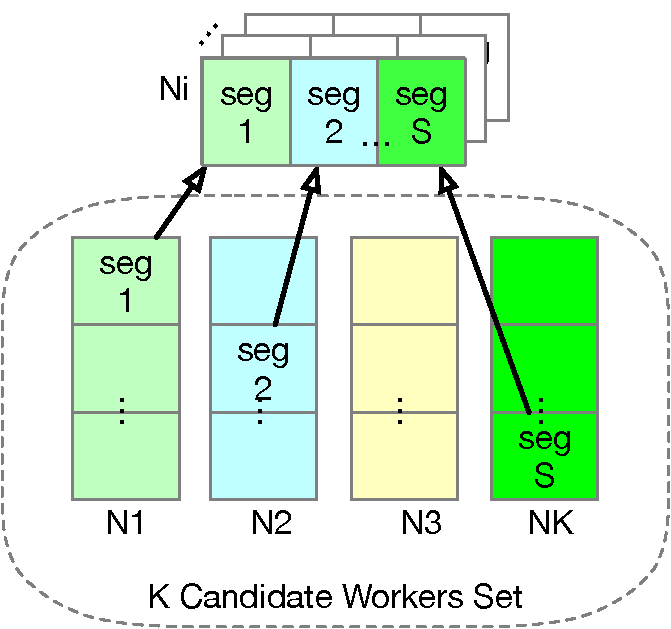
\includegraphics[width=0.225\textwidth]{pics/transfer.pdf}}
\subfigure[Segment Aggregation]{
\label{Fig.Segment sub.2}
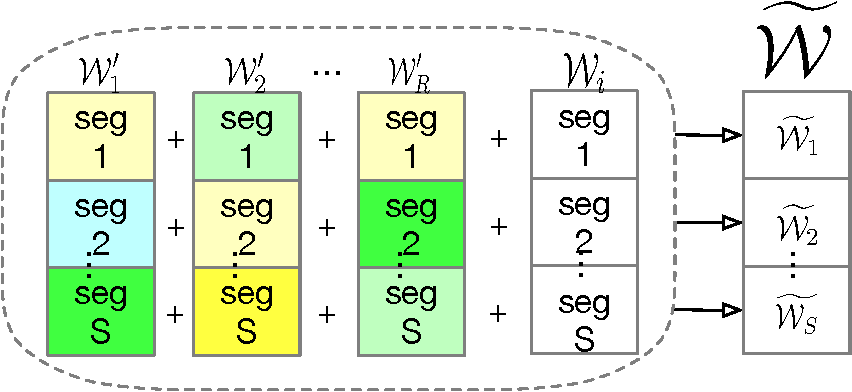
\includegraphics[width=0.225\textwidth]{pics/aggregation.pdf}}
\caption{Segment Transfer and }
\label{Fig: Segment}
\end{figure}

\subsubsection{Segmented Aggregation}
Typically the model aggregation uses weighted mean of the model parameters with the node's dataset size as weight. But in \sys, the mixed models are patched together so it is hard to set a reasonable weight for the mixed model as a whole. For such case, we use a segment-wise model aggregation in \sys.

 Assume the node $i$ has has fetched all the segments and rebuilt $R$ mixed models which we represent as $\mathcal{W}^\prime_1,\mathcal{W}^\prime_2, \dots ,\mathcal{W}^\prime_R$. Let $\mathcal{W}$ denote the model parameters of node $i$. First, we break $\mathcal{W}$ to $S$ segments using the same rule as the segmented transfer. Then for each segment $l$, we have $R$ mixed models and 1 local model to aggregate. Let $P_l$ denote the set of the nodes which provide the segment $l$(node $i$ is contained too) and $|D_j|$ denote the dataset size of node $j$, then we can aggregate segments $l$ by:
 \begin{equation}
     \widetilde{\mathcal{W}}[l] = \frac{\sum_{j\in P_l}|D_j|\mathcal{W}[l;j]}{\sum_{j\in P_l}|D_j|}
 \end{equation}

With all the aggregated segments $\widetilde{\mathcal{W}}[l]$, we can rebuild the final result by using \eqref{eq:seg_union}. And then the node can continue its training until next aggregation phase comes.

\subsection{Server Dynamic Configuration}

\subsubsection{Available Worker Updates}


\subsubsection{Fault Tolerence}
In the context of federated learning, the participating nodes are more likely to be mobile phones and embedded devices, which are often not connected to a power supply and stable network. To ensure the availability of the devices, traditional distributed systems adopt the heartbeat packet and time threshold to determine the status of the nodes. However, these methods are not applicable with federated learning for next two reasons: 1) The server has to maintain the heartbeat connection with all the participating nodes which limits the scalability of the system. 2) The computation times of each nodes vary greatly due to the difference of the computing devices and network environment.

Fortunately, the design of \sys gives us an opportunity to solve this problem decently. In the normal situation, when a node comes to the federation, it just has to register itself on the index server, pull the newest model segments to rebuild a model as its own, and then it's in. When it quits, it should wipe out its record at index server so other nodes won't request its model.

And the interesting thing is that when the node exits accidentally, it doesn't affect the federation at all. The node won't be noticed if no one requests model from this node. And if a node does randomly chooses this absent node as its target and fails to connect, it just has to select another node and report the absence to the server. Then the server know it's time to stop providing this absent node as candidate and delete the record. And if it is a false report due to the network connection, the index can be quickly rebuilt as long as the communication between the absent node and the index server reestablished. 
\section{Performance Evaluation}

%The evaluation of \sys can be divided into two parts. We develop a virtual network environment with Mininet which is able to build complex network topology and run real data transmission by virtualizing multiple kernels. The bandwidth is limited to simulate the real WAN environment and we program the virtual kernels to train and communicate according to the protocols of federated averaging algorithm and \sys. Note that in the network simulation, the kernel performs pseudo-training which only consumes time but trains nothing. On the other hand, we perform the training process on a single machine with 4x NVIDIA GTX 1080 Ti graphic cards. The training process is logically identical with the real distributed systems only but it executes the training of each node sequentially. Some details are as follows:

\subsection{Setup}

We conduct simulation experiments to evaluate our design. The evaluation can be divided into two parts. First, the stateful and synchronous nature of \sys allows us to simulate the training process sequentially, while logically, the training result is the same as the parallelized way. The training traces of each worker are then recorded, which contains the validation accuracies, training iterations, and corresponding synchronization partners. Second, we simulate the network topology and feed it with the training traces to estimate the training time. The specific settings are listed as follows:

$\triangleright$ \textit{Training settings.} We train a CNN model on CIFAR-10 dataset to evaluate the training ability of \sys. The dataset consists of  50,000 images for training and 10,000 for validation. The training data are randomly distributed among the workers without overlapping, and the validation data are shared among every worker. The CNN model is adopted from \cite{McMahan2017FL}, which is considered to be suitable for CIFAR-10 dataset. 

The models are trained on each worker using SGD algorithm with the same hyper-parameters, that a learning rate of 0.1 and a batch size of 128. The synchronization interval is set to 40, which means every worker perform SGD updates on the local model for 40 times before it communicates with others.

$\triangleright$ \textit{Network settings.} We simulate a fully connected network topology among the workers. The maximum bandwidth limit of each worker is set to be 100Mbps. Moreover, to simulate the bottleneck of WAN, we set 10Mbps as the available bandwidth between two workers.

$\triangleright$ \textit{Comparison settings.} We compare \sys and (1) traditional federated learning system with a \emph{centralized} parameter server and (2) naive \emph{gossip} approach without segmentation. To make them comparable, they are all simulated within the same network topology, and for the centralized system, we randomly choose one worker to play the role of parameter server.

The communication behavior of \sys is controlled by two parameters: \emph{model segments} as $S$ and \emph{model replica} as $R$. In our following experiments, we set $S=10$ and $R=2$ by default, that is in the synchronization phase, the model is partitioned into ten segments, and for each segment, the worker requests two replicas from other workers. The gossip approach is the special case of \sys when $S=1$, and it shares the same value of $R$ with \sys.


$\triangleright$ \textit{Performance Metrics.} The learning performance is measured by the convergence speed. We record the top-1 validation accuracies of the aggregated models at each round and then align the accuracies to the corresponding times. The time is acquired from our network simulator where the local update time is referenced from the real machine time of training with a GTX 1080 Ti graphics card, and the communication time is calculated according to the bandwidth limitations.


\subsection{Experiment Result}

We first evaluate the convergence speed and scalability of \sys in comparison to the other approaches, then we explore the advantages and disadvantages of the design of model segments and replicas and how they affect the training performance.

\subsubsection{Convergence Speed}

We present the whole training process over time, as illustrated in Fig.\ref{Fig: time_acc_30}, \sys exhibits an apparent speedup in the convergence without affecting the final validation accuracy. We also explore the scalability of these three methods by comparing the training time needed to reach a predefined accuracy goal with varying number of workers among 20, 30, and 40. According to Fig.\ref{Fig: time_acc_30}, the model reaches convergence around 82\% validation accuracy. Since the aim is not achieving the best accuracy and practically speaking, it is not worthy of spending too much time for only 1\% or 2\% accuracy gain. Thus we set 80\% as the accuracy goal. 

As illustrated in Fig.\ref{Fig: scale_time}, \sys requires the least training time to reach the given accuracy within all three cases and compared with the centralized system, the speedup of \sys increases from $2.25\times$ to $3.01\times$ with the expansion of scale. This phenomenon indicates that the decentralized federated learning is more scalable than the centralized way. Additionally, both as the decentralized approaches, \sys almost reduces the training time by half compared with the naive gossip solution.

%%%%%%%%%%%%%%%%%%%%%%%%%%%%%
\begin{figure*}[htbp]

\begin{minipage}[t]{0.32\textwidth}%%\centering
\subfigure[Convergence with 30 workers]{
\label{Fig: time_acc_30}
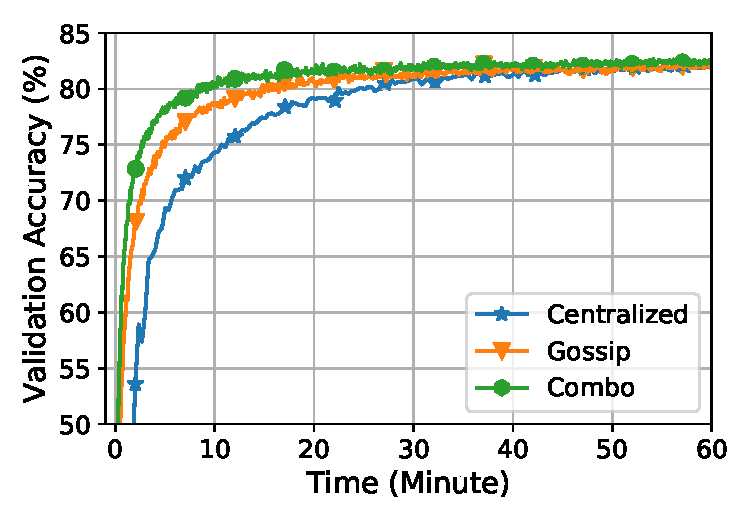
\includegraphics[width=0.9\textwidth]{pics/time_acc_30_refill.pdf}}
\\
\subfigure[Time to reach 80\% accuracy]{
\label{Fig: scale_time}
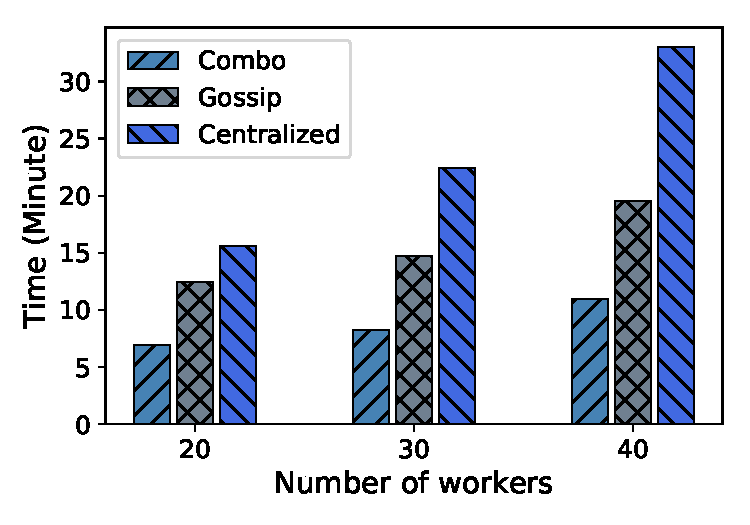
\includegraphics[width=0.9\textwidth]{pics/scale_time_refill.pdf}}

\caption{Convergence speed}
\label{Fig: acc}
\end{minipage}
\begin{minipage}[t]{0.32\linewidth}
\centering 
\subfigure[Convergence with model segments]{
\label{Fig: seg_acc}
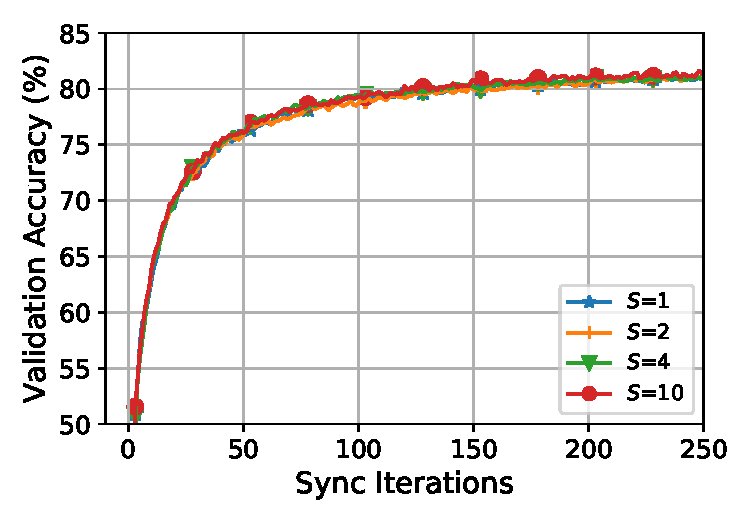
\includegraphics[width=0.9\textwidth]{pics/segment_acc_fill.pdf}}
\\
\subfigure[Sync time comparison]{
\label{Fig: seg_time}
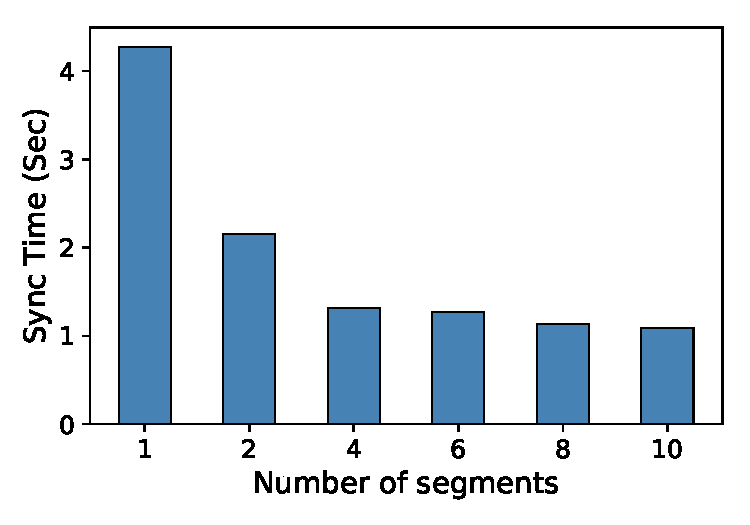
\includegraphics[width=0.9\textwidth]{pics/segment_time.pdf}}
\caption{Benefit of model segments}
\label{Fig: acc}
\end{minipage}
\begin{minipage}[t]{0.32\linewidth}
\centering 
\subfigure[Convergence with model replicas]{
\label{Fig: replica_acc}
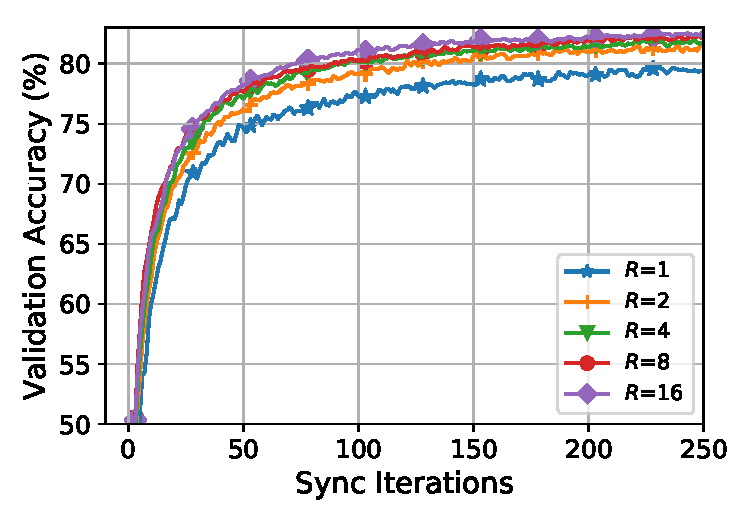
\includegraphics[width=0.9\textwidth]{pics/replica_acc_fill.pdf}}
\\
\subfigure[Time to reach 80\% accuracy]{
\label{Fig: replica_time}
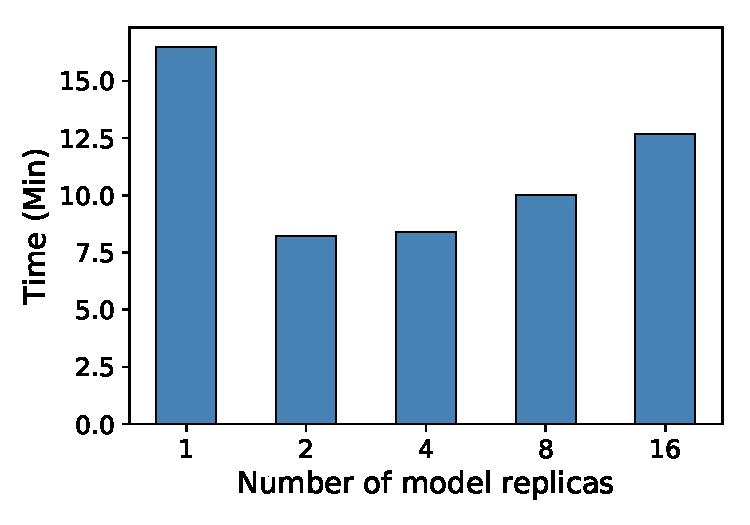
\includegraphics[width=0.9\textwidth]{pics/replica_time}}

\caption{Impact of model replicas}
\label{Fig: acc}
\end{minipage}

\end{figure*}



\subsubsection{Benefit of Model Segments}
The speedup of decentralized approaches comes from the removal of the bottleneck of the centralized server, and the advantage of \sys comes from the benefit of model segments. We train the mode with 30 workers, fix $R=2$ and vary $S$ from 1 to 10 to investigate how model segments affect the training performance.

Compared with the naive gossip solution, \sys aggregates mixed model parameters made up of multiple segments instead of the complete model. A potential concern is that the result may suffer degradation as the aggregation target is mottled and loses integrality. However, Fig.\ref{Fig: seg_acc} shows that the accuracy of the aggregated results at each synchronization iterations is not affected by the model segments at all. Partitioning the model into ten segments($S=10$) has the same convergence trend as that without partition.

While the model segments don't affect the accuracy at each iteration, the synchronization time is significantly reduced. As illustrated in Fig.\ref{Fig: seg_time}, by simply splitting the model parameters into two segments can reduce the synchronization time by half. This is because when $S=2$, the original transmission quantity is divided into two parts and fed into $2\times$ more links. When the bandwidth is not exhausted, the sending and receiving time can be reduced almost proportionally. However, when $S\geq 6$, the bandwidth is already fully exploited, increasing the number of segments will not improve the time consumption then.


\subsubsection{Impact of Model Replicas}

Next, we evaluate the impact of model replica, which controls the overall information quantity that the workers send and receive at each synchronization iterations. Similar to the previous settings, we fix $S=10$ and vary $R$ from 1 to 16.

As we discussed in the convergence analysis of \sys, the more information a worker receives, the better aggregation result it will get. When the worker receives all the model replicas from other peers, \sys becomes the All-reduce structure and achieves the same training result as the centralized approach. The analysis is validated by Fig.\ref{Fig: replica_acc} that with the increase of the number of model replicas, the accuracy of each iteration becomes better. However, the improvement is not unlimited. We can see that there is no significant gap between $R=8$ and $16$ in the convergence trend and result. This reflects the redundancy of All-reduce structure that the worker doesn't have to collect all the external models to train a high-quality model.

However, as the bandwidth of worker is fully utilized with model segments, increasing $R$ leads to the proportional growth of the transmission workload. Thus there exists a tradeoff, a larger $R$ increases the convergence rate on synchronization iterations but also the synchronization time. We compare the training time needed to reach 80\% validation accuracy with different $R$ as shown in Fig.\ref{Fig: replica_time}. Increasing $R=1$ to $2$ leads to a rapid reduction of the required training time as it drastically reduces the iterations needed to achieve target accuracy goal, which is also illustrated in Fig.\ref{Fig: replica_acc}. However, if we continue to increase $R$, the growth of the training time exceeds the reduction of the iterations and slows down the convergence speed.














\section{Conclusion}
One of the most challenging problem of federated learning is the poor network connection as the workers are geo-distributed and connected with slow WAN. To avoid the drawback of high possibility network congestion in centralized parameter sever architecture, which is adopted in today's FL systems, we explore the possibility of decentralized FL solution, called \sys. Taking the insight that the peer-to-peer bandwidth is much smaller than the worker's maximum network capacity, \sys could fully utilize the bandwidth by saturating the network with segmented gossip aggregation. The experiments show that \sys significantly reduces the training time and remains good convergence performance.
%but still has good convergence.
\section{Analysis}

\newcommand{\wti}{W_{t,i}}
\newcommand{\wtj}{W_{t,j}}
\newcommand{\wt}{W_{t}}
\newcommand{\norm}[1]{\Vert #1 \Vert_{1}}


\begin{equation}
\begin{split}
	\Vert \wti - W^*\Vert & = \Vert \wti -\wt + \wt - W^*\Vert \\
                      & \leq \Vert \wti -\wt \Vert + \Vert \wt - W^* \Vert \\
                      & \leq \Vert \wti -\wt \Vert + \rho	
\end{split}
\end{equation}

\begin{equation}
\begin{split}
	\norm{\wt -W^*}  & = \norm{\sum_{j\in N} \frac{|D_j|\widetilde{\wtj}}{|D|} - W^*}  \\
	& = \norm{\sum_{j\in N} \frac{|D_j|\tilde{\wtj}}{|D|} - \sum_{j\in N} \frac{|D_j|W^*}{|D|}} \\
	& = \norm{ \sum_{j\in N} \frac{|D_j|}{|D|} ( \widetilde{\wtj} -W^* ) } \\
	& \leq \sum_{j\in N} \frac{|D_j|}{|D|} \norm{\widetilde{\wtj} -W^* } \\
	& \leq \norm{\widetilde{W_{t,\hat{j}} } - W^*}
\end{split}
\end{equation}

Where $\hat{j} = argmax \sum_{j\in N} \frac{|D_j|}{|D|} \norm{\widetilde{W_{t,\hat{j}} } - W^*}$ 



\bibliographystyle{IEEEtran}
\bibliography{ref.bib}


%\section{Introduction}
%\label{sec:introduction}
%\PARstart{T}{his} document is a template for \LaTeX. If you are 
%reading a paper or PDF version of this document, please download the 
%electronic file, trans\_jour.tex, from the IEEE Web site at \underline
%{http://ieeeauthorcenter.ieee.org/create-your-ieee-article/}\break\underline{use-authoring-tools-and-ieee-article-templates/ieee-article-}\break\underline{templates/} so you can use it to prepare your manuscript. If 
%you would prefer to use LaTeX, download IEEE's LaTeX style and sample files 
%from the same Web page. You can also explore using the Overleaf editor at 
%\underline
%{https://www.overleaf.com/blog/278-how-to-use-overleaf-}\break\underline{with-ieee-collabratec-your-quick-guide-to-getting-started}\break\underline{\#.xsVp6tpPkrKM9}
%
%If your paper is intended for a conference, please contact your conference 
%editor concerning acceptable word processor formats for your particular 
%conference. 
%
%IEEE will do the final formatting of your paper. If your paper is intended 
%for a conference, please observe the conference page limits. 
%
%\subsection{Abbreviations and Acronyms}
%Define abbreviations and acronyms the first time they are used in the text, 
%even after they have already been defined in the abstract. Abbreviations 
%such as IEEE, SI, ac, and dc do not have to be defined. Abbreviations that 
%incorporate periods should not have spaces: write ``C.N.R.S.,'' not ``C. N. 
%R. S.'' Do not use abbreviations in the title unless they are unavoidable 
%(for example, ``IEEE'' in the title of this article).
%
%\subsection{Other Recommendations}
%Use one space after periods and colons. Hyphenate complex modifiers: 
%``zero-field-cooled magnetization.'' Avoid dangling participles, such as, 
%``Using \eqref{eq}, the potential was calculated.'' [It is not clear who or what 
%used \eqref{eq}.] Write instead, ``The potential was calculated by using \eqref{eq},'' or 
%``Using \eqref{eq}, we calculated the potential.''
%
%Use a zero before decimal points: ``0.25,'' not ``.25.'' Use 
%``cm$^{3}$,'' not ``cc.'' Indicate sample dimensions as ``0.1 cm 
%$\times $ 0.2 cm,'' not ``0.1 $\times $ 0.2 cm$^{2}$.'' The 
%abbreviation for ``seconds'' is ``s,'' not ``sec.'' Use 
%``Wb/m$^{2}$'' or ``webers per square meter,'' not 
%``webers/m$^{2}$.'' When expressing a range of values, write ``7 to 
%9'' or ``7--9,'' not ``7$\sim $9.''
%
%A parenthetical statement at the end of a sentence is punctuated outside of 
%the closing parenthesis (like this). (A parenthetical sentence is punctuated 
%within the parentheses.) In American English, periods and commas are within 
%quotation marks, like ``this period.'' Other punctuation is ``outside''! 
%Avoid contractions; for example, write ``do not'' instead of ``don't.'' The 
%serial comma is preferred: ``A, B, and C'' instead of ``A, B and C.''
%
%If you wish, you may write in the first person singular or plural and use 
%the active voice (``I observed that $\ldots$'' or ``We observed that $\ldots$'' 
%instead of ``It was observed that $\ldots$''). Remember to check spelling. If 
%your native language is not English, please get a native English-speaking 
%colleague to carefully proofread your paper.
%
%Try not to use too many typefaces in the same article. You're writing
%scholarly papers, not ransom notes. Also please remember that MathJax
%can't handle really weird typefaces.
%
%\subsection{Equations}
%Number equations consecutively with equation numbers in parentheses flush 
%with the right margin, as in \eqref{eq}. To make your equations more 
%compact, you may use the solidus (~/~), the exp function, or appropriate 
%exponents. Use parentheses to avoid ambiguities in denominators. Punctuate 
%equations when they are part of a sentence, as in
%\begin{equation}E=mc^2.\label{eq}\end{equation}
%
%Be sure that the symbols in your equation have been defined before the 
%equation appears or immediately following. Italicize symbols ($T$ might refer 
%to temperature, but T is the unit tesla). Refer to ``\eqref{eq},'' not ``Eq. \eqref{eq}'' 
%or ``equation \eqref{eq},'' except at the beginning of a sentence: ``Equation \eqref{eq} 
%is $\ldots$ .''
%
%\subsection{\LaTeX-Specific Advice}
%
%Please use ``soft'' (e.g., \verb|\eqref{Eq}|) cross references instead
%of ``hard'' references (e.g., \verb|(1)|). That will make it possible
%to combine sections, add equations, or change the order of figures or
%citations without having to go through the file line by line.
%
%Please don't use the \verb|{eqnarray}| equation environment. Use
%\verb|{align}| or \verb|{IEEEeqnarray}| instead. The \verb|{eqnarray}|
%environment leaves unsightly spaces around relation symbols.
%
%Please note that the \verb|{subequations}| environment in {\LaTeX}
%will increment the main equation counter even when there are no
%equation numbers displayed. If you forget that, you might write an
%article in which the equation numbers skip from (17) to (20), causing
%the copy editors to wonder if you've discovered a new method of
%counting.
%
%{\BibTeX} does not work by magic. It doesn't get the bibliographic
%data from thin air but from .bib files. If you use {\BibTeX} to produce a
%bibliography you must send the .bib files. 
%
%{\LaTeX} can't read your mind. If you assign the same label to a
%subsubsection and a table, you might find that Table I has been cross
%referenced as Table IV-B3. 
%
%{\LaTeX} does not have precognitive abilities. If you put a
%\verb|\label| command before the command that updates the counter it's
%supposed to be using, the label will pick up the last counter to be
%cross referenced instead. In particular, a \verb|\label| command
%should not go before the caption of a figure or a table.
%
%Do not use \verb|\nonumber| inside the \verb|{array}| environment. It
%will not stop equation numbers inside \verb|{array}| (there won't be
%any anyway) and it might stop a wanted equation number in the
%surrounding equation.
%
%\section{Units}
%Use either SI (MKS) or CGS as primary units. (SI units are strongly 
%encouraged.) English units may be used as secondary units (in parentheses). 
%This applies to papers in data storage. For example, write ``15 
%Gb/cm$^{2}$ (100 Gb/in$^{2})$.'' An exception is when 
%English units are used as identifiers in trade, such as ``3\textonehalf-in 
%disk drive.'' Avoid combining SI and CGS units, such as current in amperes 
%and magnetic field in oersteds. This often leads to confusion because 
%equations do not balance dimensionally. If you must use mixed units, clearly 
%state the units for each quantity in an equation.
%
%The SI unit for magnetic field strength $H$ is A/m. However, if you wish to use 
%units of T, either refer to magnetic flux density $B$ or magnetic field 
%strength symbolized as $\mu _{0}H$. Use the center dot to separate 
%compound units, e.g., ``A$\cdot $m$^{2}$.''
%
%\section{Some Common Mistakes}
%The word ``data'' is plural, not singular. The subscript for the 
%permeability of vacuum $\mu _{0}$ is zero, not a lowercase letter 
%``o.'' The term for residual magnetization is ``remanence''; the adjective 
%is ``remanent''; do not write ``remnance'' or ``remnant.'' Use the word 
%``micrometer'' instead of ``micron.'' A graph within a graph is an 
%``inset,'' not an ``insert.'' The word ``alternatively'' is preferred to the 
%word ``alternately'' (unless you really mean something that alternates). Use 
%the word ``whereas'' instead of ``while'' (unless you are referring to 
%simultaneous events). Do not use the word ``essentially'' to mean 
%``approximately'' or ``effectively.'' Do not use the word ``issue'' as a 
%euphemism for ``problem.'' When compositions are not specified, separate 
%chemical symbols by en-dashes; for example, ``NiMn'' indicates the 
%intermetallic compound Ni$_{0.5}$Mn$_{0.5}$ whereas 
%``Ni--Mn'' indicates an alloy of some composition 
%Ni$_{x}$Mn$_{1-x}$.
%
%\Figure[t!](topskip=0pt, botskip=0pt, midskip=0pt){fig1.png}
%{Magnetization as a function of applied field.
%It is good practice to explain the significance of the figure in the caption.\label{fig1}}
%
%Be aware of the different meanings of the homophones ``affect'' (usually a 
%verb) and ``effect'' (usually a noun), ``complement'' and ``compliment,'' 
%``discreet'' and ``discrete,'' ``principal'' (e.g., ``principal 
%investigator'') and ``principle'' (e.g., ``principle of measurement''). Do 
%not confuse ``imply'' and ``infer.'' 
%
%Prefixes such as ``non,'' ``sub,'' ``micro,'' ``multi,'' and ``ultra'' are 
%not independent words; they should be joined to the words they modify, 
%usually without a hyphen. There is no period after the ``et'' in the Latin 
%abbreviation ``\emph{et al.}'' (it is also italicized). The abbreviation ``i.e.,'' means 
%``that is,'' and the abbreviation ``e.g.,'' means ``for example'' (these 
%abbreviations are not italicized).
%
%A general IEEE styleguide is available at \underline{http://www.ieee.org/}\break\underline{authortools}.
%
%\section{Guidelines for Graphics Preparation and Submission}
%\label{sec:guidelines}
%
%\subsection{Types of Graphics}
%The following list outlines the different types of graphics published in 
%IEEE journals. They are categorized based on their construction, and use of 
%color/shades of gray:
%
%\subsubsection{Color/Grayscale figures}
%{Figures that are meant to appear in color, or shades of black/gray. Such 
%figures may include photographs, illustrations, multicolor graphs, and 
%flowcharts.}
%
%\subsubsection{Line Art figures}
%{Figures that are composed of only black lines and shapes. These figures 
%should have no shades or half-tones of gray, only black and white.}
%
%\subsubsection{Author photos}
%{Head and shoulders shots of authors that appear at the end of our papers. }
%
%\subsubsection{Tables}
%{Data charts which are typically black and white, but sometimes include 
%color.}
%
%\begin{table}
%\caption{Units for Magnetic Properties}
%\label{table}
%\setlength{\tabcolsep}{3pt}
%\begin{tabular}{|p{25pt}|p{75pt}|p{115pt}|}
%\hline
%Symbol& 
%Quantity& 
%Conversion from Gaussian and \par CGS EMU to SI $^{\mathrm{a}}$ \\
%\hline
%$\Phi $& 
%magnetic flux& 
%1 Mx $\to  10^{-8}$ Wb $= 10^{-8}$ V$\cdot $s \\
%$B$& 
%magnetic flux density, \par magnetic induction& 
%1 G $\to  10^{-4}$ T $= 10^{-4}$ Wb/m$^{2}$ \\
%$H$& 
%magnetic field strength& 
%1 Oe $\to  10^{3}/(4\pi )$ A/m \\
%$m$& 
%magnetic moment& 
%1 erg/G $=$ 1 emu \par $\to 10^{-3}$ A$\cdot $m$^{2} = 10^{-3}$ J/T \\
%$M$& 
%magnetization& 
%1 erg/(G$\cdot $cm$^{3}) =$ 1 emu/cm$^{3}$ \par $\to 10^{3}$ A/m \\
%4$\pi M$& 
%magnetization& 
%1 G $\to  10^{3}/(4\pi )$ A/m \\
%$\sigma $& 
%specific magnetization& 
%1 erg/(G$\cdot $g) $=$ 1 emu/g $\to $ 1 A$\cdot $m$^{2}$/kg \\
%$j$& 
%magnetic dipole \par moment& 
%1 erg/G $=$ 1 emu \par $\to 4\pi \times  10^{-10}$ Wb$\cdot $m \\
%$J$& 
%magnetic polarization& 
%1 erg/(G$\cdot $cm$^{3}) =$ 1 emu/cm$^{3}$ \par $\to 4\pi \times  10^{-4}$ T \\
%$\chi , \kappa $& 
%susceptibility& 
%1 $\to  4\pi $ \\
%$\chi_{\rho }$& 
%mass susceptibility& 
%1 cm$^{3}$/g $\to  4\pi \times  10^{-3}$ m$^{3}$/kg \\
%$\mu $& 
%permeability& 
%1 $\to  4\pi \times  10^{-7}$ H/m \par $= 4\pi \times  10^{-7}$ Wb/(A$\cdot $m) \\
%$\mu_{r}$& 
%relative permeability& 
%$\mu \to \mu_{r}$ \\
%$w, W$& 
%energy density& 
%1 erg/cm$^{3} \to  10^{-1}$ J/m$^{3}$ \\
%$N, D$& 
%demagnetizing factor& 
%1 $\to  1/(4\pi )$ \\
%\hline
%\multicolumn{3}{p{251pt}}{Vertical lines are optional in tables. Statements that serve as captions for 
%the entire table do not need footnote letters. }\\
%\multicolumn{3}{p{251pt}}{$^{\mathrm{a}}$Gaussian units are the same as cg emu for magnetostatics; Mx 
%$=$ maxwell, G $=$ gauss, Oe $=$ oersted; Wb $=$ weber, V $=$ volt, s $=$ 
%second, T $=$ tesla, m $=$ meter, A $=$ ampere, J $=$ joule, kg $=$ 
%kilogram, H $=$ henry.}
%\end{tabular}
%\label{tab1}
%\end{table}
%
%\subsection{Multipart figures}
%Figures compiled of more than one sub-figure presented side-by-side, or 
%stacked. If a multipart figure is made up of multiple figure
%types (one part is lineart, and another is grayscale or color) the figure 
%should meet the stricter guidelines.
%
%\subsection{File Formats For Graphics}\label{formats}
%Format and save your graphics using a suitable graphics processing program 
%that will allow you to create the images as PostScript (PS), Encapsulated 
%PostScript (.EPS), Tagged Image File Format (.TIFF), Portable Document 
%Format (.PDF), Portable Network Graphics (.PNG), or Metapost (.MPS), sizes them, and adjusts 
%the resolution settings. When 
%submitting your final paper, your graphics should all be submitted 
%individually in one of these formats along with the manuscript.
%
%\subsection{Sizing of Graphics}
%Most charts, graphs, and tables are one column wide (3.5 inches/88 
%millimeters/21 picas) or page wide (7.16 inches/181 millimeters/43 
%picas). The maximum depth a graphic can be is 8.5 inches (216 millimeters/54
%picas). When choosing the depth of a graphic, please allow space for a 
%caption. Figures can be sized between column and page widths if the author 
%chooses, however it is recommended that figures are not sized less than 
%column width unless when necessary. 
%
%There is currently one publication with column measurements that do not 
%coincide with those listed above. Proceedings of the IEEE has a column 
%measurement of 3.25 inches (82.5 millimeters/19.5 picas). 
%
%The final printed size of author photographs is exactly
%1 inch wide by 1.25 inches tall (25.4 millimeters$\,\times\,$31.75 millimeters/6 
%picas$\,\times\,$7.5 picas). Author photos printed in editorials measure 1.59 inches 
%wide by 2 inches tall (40 millimeters$\,\times\,$50 millimeters/9.5 picas$\,\times\,$12 
%picas).
%
%\subsection{Resolution }
%The proper resolution of your figures will depend on the type of figure it 
%is as defined in the ``Types of Figures'' section. Author photographs, 
%color, and grayscale figures should be at least 300dpi. Line art, including 
%tables should be a minimum of 600dpi.
%
%\subsection{Vector Art}
%In order to preserve the figures' integrity across multiple computer 
%platforms, we accept files in the following formats: .EPS/.PDF/.PS. All 
%fonts must be embedded or text converted to outlines in order to achieve the 
%best-quality results.
%
%\subsection{Color Space}
%The term color space refers to the entire sum of colors that can be 
%represented within the said medium. For our purposes, the three main color 
%spaces are Grayscale, RGB (red/green/blue) and CMYK 
%(cyan/magenta/yellow/black). RGB is generally used with on-screen graphics, 
%whereas CMYK is used for printing purposes.
%
%All color figures should be generated in RGB or CMYK color space. Grayscale 
%images should be submitted in Grayscale color space. Line art may be 
%provided in grayscale OR bitmap colorspace. Note that ``bitmap colorspace'' 
%and ``bitmap file format'' are not the same thing. When bitmap color space 
%is selected, .TIF/.TIFF/.PNG are the recommended file formats.
%
%\subsection{Accepted Fonts Within Figures}
%When preparing your graphics IEEE suggests that you use of one of the 
%following Open Type fonts: Times New Roman, Helvetica, Arial, Cambria, and 
%Symbol. If you are supplying EPS, PS, or PDF files all fonts must be 
%embedded. Some fonts may only be native to your operating system; without 
%the fonts embedded, parts of the graphic may be distorted or missing.
%
%A safe option when finalizing your figures is to strip out the fonts before 
%you save the files, creating ``outline'' type. This converts fonts to 
%artwork what will appear uniformly on any screen.
%
%\subsection{Using Labels Within Figures}
%
%\subsubsection{Figure Axis labels }
%Figure axis labels are often a source of confusion. Use words rather than 
%symbols. As an example, write the quantity ``Magnetization,'' or 
%``Magnetization M,'' not just ``M.'' Put units in parentheses. Do not label 
%axes only with units. As in Fig. 1, for example, write ``Magnetization 
%(A/m)'' or ``Magnetization (A$\cdot$m$^{-1}$),'' not just ``A/m.'' Do not label axes with a ratio of quantities and 
%units. For example, write ``Temperature (K),'' not ``Temperature/K.'' 
%
%Multipliers can be especially confusing. Write ``Magnetization (kA/m)'' or 
%``Magnetization (10$^{3}$ A/m).'' Do not write ``Magnetization 
%(A/m)$\,\times\,$1000'' because the reader would not know whether the top 
%axis label in Fig. 1 meant 16000 A/m or 0.016 A/m. Figure labels should be 
%legible, approximately 8 to 10 point type.
%
%\subsubsection{Subfigure Labels in Multipart Figures and Tables}
%Multipart figures should be combined and labeled before final submission. 
%Labels should appear centered below each subfigure in 8 point Times New 
%Roman font in the format of (a) (b) (c). 
%
%\subsection{File Naming}
%Figures (line artwork or photographs) should be named starting with the 
%first 5 letters of the author's last name. The next characters in the 
%filename should be the number that represents the sequential 
%location of this image in your article. For example, in author 
%``Anderson's'' paper, the first three figures would be named ander1.tif, 
%ander2.tif, and ander3.ps.
%
%Tables should contain only the body of the table (not the caption) and 
%should be named similarly to figures, except that `.t' is inserted 
%in-between the author's name and the table number. For example, author 
%Anderson's first three tables would be named ander.t1.tif, ander.t2.ps, 
%ander.t3.eps.
%
%Author photographs should be named using the first five characters of the 
%pictured author's last name. For example, four author photographs for a 
%paper may be named: oppen.ps, moshc.tif, chen.eps, and duran.pdf.
%
%If two authors or more have the same last name, their first initial(s) can 
%be substituted for the fifth, fourth, third$\ldots$ letters of their surname 
%until the degree where there is differentiation. For example, two authors 
%Michael and Monica Oppenheimer's photos would be named oppmi.tif, and 
%oppmo.eps.
%
%\subsection{Referencing a Figure or Table Within Your Paper}
%When referencing your figures and tables within your paper, use the 
%abbreviation ``Fig.'' even at the beginning of a sentence. Do not abbreviate 
%``Table.'' Tables should be numbered with Roman Numerals.
%
%\subsection{Checking Your Figures: The IEEE Graphics Analyzer}
%The IEEE Graphics Analyzer enables authors to pre-screen their graphics for 
%compliance with IEEE Access standards before submission. 
%The online tool, located at
%\underline{http://graphicsqc.ieee.org/}, allows authors to 
%upload their graphics in order to check that each file is the correct file 
%format, resolution, size and colorspace; that no fonts are missing or 
%corrupt; that figures are not compiled in layers or have transparency, and 
%that they are named according to the IEEE Access naming 
%convention. At the end of this automated process, authors are provided with 
%a detailed report on each graphic within the web applet, as well as by 
%email.
%
%For more information on using the Graphics Analyzer or any other graphics 
%related topic, contact the IEEE Graphics Help Desk by e-mail at 
%graphics@ieee.org.
%
%\subsection{Submitting Your Graphics}
%Because IEEE will do the final formatting of your paper,
%you do not need to position figures and tables at the top and bottom of each 
%column. In fact, all figures, figure captions, and tables can be placed at 
%the end of your paper. In addition to, or even in lieu of submitting figures 
%within your final manuscript, figures should be submitted individually, 
%separate from the manuscript in one of the file formats listed above in 
%Section \ref{formats}. Place figure captions below the figures; place table titles 
%above the tables. Please do not include captions as part of the figures, or 
%put them in ``text boxes'' linked to the figures. Also, do not place borders 
%around the outside of your figures.
%
%\subsection{Color Processing/Printing in IEEE Journals}
%All IEEE Transactions, Journals, and Letters allow an author to publish 
%color figures on IEEE Xplore\textregistered\ at no charge, and automatically 
%convert them to grayscale for print versions. In most journals, figures and 
%tables may alternatively be printed in color if an author chooses to do so. 
%Please note that this service comes at an extra expense to the author. If 
%you intend to have print color graphics, include a note with your final 
%paper indicating which figures or tables you would like to be handled that 
%way, and stating that you are willing to pay the additional fee.
%
%\section{Conclusion}
%A conclusion section is not required. Although a conclusion may review the 
%main points of the paper, do not replicate the abstract as the conclusion. A 
%conclusion might elaborate on the importance of the work or suggest 
%applications and extensions. 
%
%\appendices
%
%Appendixes, if needed, appear before the acknowledgment.
%
%\section*{Acknowledgment}
%
%The preferred spelling of the word ``acknowledgment'' in American English is 
%without an ``e'' after the ``g.'' Use the singular heading even if you have 
%many acknowledgments. Avoid expressions such as ``One of us (S.B.A.) would 
%like to thank $\ldots$ .'' Instead, write ``F. A. Author thanks $\ldots$ .'' In most 
%cases, sponsor and financial support acknowledgments are placed in the 
%unnumbered footnote on the first page, not here.
%
%\section*{References and Footnotes}
%
%\subsection{References}
%References need not be cited in text. When they are, they appear on the 
%line, in square brackets, inside the punctuation. Multiple references are 
%each numbered with separate brackets. When citing a section in a book, 
%please give the relevant page numbers. In text, refer simply to the 
%reference number. Do not use ``Ref.'' or ``reference'' except at the 
%beginning of a sentence: ``Reference \cite{b3} shows $\ldots$ .'' Please do not use 
%automatic endnotes in \emph{Word}, rather, type the reference list at the end of the 
%paper using the ``References'' style.
%
%Reference numbers are set flush left and form a column of their own, hanging 
%out beyond the body of the reference. The reference numbers are on the line, 
%enclosed in square brackets. In all references, the given name of the author 
%or editor is abbreviated to the initial only and precedes the last name. Use 
%them all; use \emph{et al.} only if names are not given. Use commas around Jr., 
%Sr., and III in names. Abbreviate conference titles. When citing IEEE 
%transactions, provide the issue number, page range, volume number, year, 
%and/or month if available. When referencing a patent, provide the day and 
%the month of issue, or application. References may not include all 
%information; please obtain and include relevant information. Do not combine 
%references. There must be only one reference with each number. If there is a 
%URL included with the print reference, it can be included at the end of the 
%reference. 
%
%Other than books, capitalize only the first word in a paper title, except 
%for proper nouns and element symbols. For papers published in translation 
%journals, please give the English citation first, followed by the original 
%foreign-language citation See the end of this document for formats and 
%examples of common references. For a complete discussion of references and 
%their formats, see the IEEE style manual at
%\underline{http://www.ieee.org/authortools}.
%
%\subsection{Footnotes}
%Number footnotes separately in superscript numbers.\footnote{It is recommended that footnotes be avoided (except for 
%the unnumbered footnote with the receipt date on the first page). Instead, 
%try to integrate the footnote information into the text.} Place the actual 
%footnote at the bottom of the column in which it is cited; do not put 
%footnotes in the reference list (endnotes). Use letters for table footnotes 
%(see Table \ref{table}).
%
%\section{Submitting Your Paper for Review}
%
%\subsection{Final Stage}
%When you submit your final version (after your paper has been accepted), 
%print it in two-column format, including figures and tables. You must also 
%send your final manuscript on a disk, via e-mail, or through a Web 
%manuscript submission system as directed by the society contact. You may use 
%\emph{Zip} for large files, or compress files using \emph{Compress, Pkzip, Stuffit,} or \emph{Gzip.} 
%
%Also, send a sheet of paper or PDF with complete contact information for all 
%authors. Include full mailing addresses, telephone numbers, fax numbers, and 
%e-mail addresses. This information will be used to send each author a 
%complimentary copy of the journal in which the paper appears. In addition, 
%designate one author as the ``corresponding author.'' This is the author to 
%whom proofs of the paper will be sent. Proofs are sent to the corresponding 
%author only.
%
%\subsection{Review Stage Using ScholarOne\textregistered\ Manuscripts}
%Contributions to the Transactions, Journals, and Letters may be submitted 
%electronically on IEEE's on-line manuscript submission and peer-review 
%system, ScholarOne\textregistered\ Manuscripts. You can get a listing of the 
%publications that participate in ScholarOne at 
%\underline{http://www.ieee.org/publications\_standards/publications/}\break\underline{authors/authors\_submission.html}.
%First check if you have an existing account. If there is none, please create 
%a new account. After logging in, go to your Author Center and click ``Submit 
%First Draft of a New Manuscript.'' 
%
%Along with other information, you will be asked to select the subject from a 
%pull-down list. Depending on the journal, there are various steps to the 
%submission process; you must complete all steps for a complete submission. 
%At the end of each step you must click ``Save and Continue''; just uploading 
%the paper is not sufficient. After the last step, you should see a 
%confirmation that the submission is complete. You should also receive an 
%e-mail confirmation. For inquiries regarding the submission of your paper on 
%ScholarOne Manuscripts, please contact oprs-support@ieee.org or call +1 732 
%465 5861.
%
%ScholarOne Manuscripts will accept files for review in various formats. 
%Please check the guidelines of the specific journal for which you plan to 
%submit.
%
%You will be asked to file an electronic copyright form immediately upon 
%completing the submission process (authors are responsible for obtaining any 
%security clearances). Failure to submit the electronic copyright could 
%result in publishing delays later. You will also have the opportunity to 
%designate your article as ``open access'' if you agree to pay the IEEE open 
%access fee. 
%
%\subsection{Final Stage Using ScholarOne Manuscripts}
%Upon acceptance, you will receive an email with specific instructions 
%regarding the submission of your final files. To avoid any delays in 
%publication, please be sure to follow these instructions. Most journals 
%require that final submissions be uploaded through ScholarOne Manuscripts, 
%although some may still accept final submissions via email. Final 
%submissions should include source files of your accepted manuscript, high 
%quality graphic files, and a formatted pdf file. If you have any questions 
%regarding the final submission process, please contact the administrative 
%contact for the journal. 
%
%In addition to this, upload a file with complete contact information for all 
%authors. Include full mailing addresses, telephone numbers, fax numbers, and 
%e-mail addresses. Designate the author who submitted the manuscript on 
%ScholarOne Manuscripts as the ``corresponding author.'' This is the only 
%author to whom proofs of the paper will be sent. 
%
%\subsection{Copyright Form}
%Authors must submit an electronic IEEE Copyright Form (eCF) upon submitting 
%their final manuscript files. You can access the eCF system through your 
%manuscript submission system or through the Author Gateway. You are 
%responsible for obtaining any necessary approvals and/or security 
%clearances. For additional information on intellectual property rights, 
%visit the IEEE Intellectual Property Rights department web page at 
%\underline{http://www.ieee.org/publications\_standards/publications/}\break\underline{rights/index.html}. 
%
%\section{IEEE Publishing Policy}
%The general IEEE policy requires that authors should only submit original 
%work that has neither appeared elsewhere for publication, nor is under 
%review for another refereed publication. The submitting author must disclose 
%all prior publication(s) and current submissions when submitting a 
%manuscript. Do not publish ``preliminary'' data or results. The submitting 
%author is responsible for obtaining agreement of all coauthors and any 
%consent required from employers or sponsors before submitting an article. 
%The IEEE Access Department strongly discourages courtesy 
%authorship; it is the obligation of the authors to cite only relevant prior 
%work.
%
%The IEEE Access Department does not publish conference 
%records or proceedings, but can publish articles related to conferences that 
%have undergone rigorous peer review. Minimally, two reviews are required for 
%every article submitted for peer review.
%
%\section{Publication Principles}
%The two types of contents of that are published are; 1) peer-reviewed and 2) 
%archival. The Access Department publishes scholarly 
%articles of archival value as well as tutorial expositions and critical 
%reviews of classical subjects and topics of current interest. 
%
%Authors should consider the following points:
%
%\begin{enumerate}
%\item Technical papers submitted for publication must advance the state of knowledge and must cite relevant prior work. 
%\item The length of a submitted paper should be commensurate with the importance, or appropriate to the complexity, of the work. For example, an obvious extension of previously published work might not be appropriate for publication or might be adequately treated in just a few pages.
%\item Authors must convince both peer reviewers and the editors of the scientific and technical merit of a paper; the standards of proof are higher when extraordinary or unexpected results are reported. 
%\item Because replication is required for scientific progress, papers submitted for publication must provide sufficient information to allow readers to perform similar experiments or calculations and 
%use the reported results. Although not everything need be disclosed, a paper 
%must contain new, useable, and fully described information. For example, a 
%specimen's chemical composition need not be reported if the main purpose of 
%a paper is to introduce a new measurement technique. Authors should expect 
%to be challenged by reviewers if the results are not supported by adequate 
%data and critical details.
%\item Papers that describe ongoing work or announce the latest technical achievement, which are suitable for presentation at a professional conference, may not be appropriate for publication.
%\end{enumerate}

% \section{Reference Examples}

% \begin{itemize}

% \item \emph{Basic format for books:}\\
% J. K. Author, ``Title of chapter in the book,'' in \emph{Title of His Published Book, x}th ed. City of Publisher, (only U.S. State), Country: Abbrev. of Publisher, year, ch. $x$, sec. $x$, pp. \emph{xxx--xxx.}\\
% See \cite{b1,b2}.

% \item \emph{Basic format for periodicals:}\\
% J. K. Author, ``Name of paper,'' \emph{Abbrev. Title of Periodical}, vol. \emph{x, no}. $x, $pp\emph{. xxx--xxx, }Abbrev. Month, year, DOI. 10.1109.\emph{XXX}.123456.\\
% See \cite{b3}--\cite{b5}.

% \item \emph{Basic format for reports:}\\
% J. K. Author, ``Title of report,'' Abbrev. Name of Co., City of Co., Abbrev. State, Country, Rep. \emph{xxx}, year.\\
% See \cite{b6,b7}.

% \item \emph{Basic format for handbooks:}\\
% \emph{Name of Manual/Handbook, x} ed., Abbrev. Name of Co., City of Co., Abbrev. State, Country, year, pp. \emph{xxx--xxx.}\\
% See \cite{b8,b9}.

% \item \emph{Basic format for books (when available online):}\\
% J. K. Author, ``Title of chapter in the book,'' in \emph{Title of
% Published Book}, $x$th ed. City of Publisher, State, Country: Abbrev.
% of Publisher, year, ch. $x$, sec. $x$, pp. \emph{xxx--xxx}. [Online].
% Available: \underline{http://www.web.com}\\
% See \cite{b10}--\cite{b13}.

% \item \emph{Basic format for journals (when available online):}\\
% J. K. Author, ``Name of paper,'' \emph{Abbrev. Title of Periodical}, vol. $x$, no. $x$, pp. \emph{xxx--xxx}, Abbrev. Month, year. Accessed on: Month, Day, year, DOI: 10.1109.\emph{XXX}.123456, [Online].\\
% See \cite{b14}--\cite{b16}.

% \item \emph{Basic format for papers presented at conferences (when available online): }\\
% J.K. Author. (year, month). Title. presented at abbrev. conference title. [Type of Medium]. Available: site/path/file\\
% See \cite{b17}.

% \item \emph{Basic format for reports and handbooks (when available online):}\\
% J. K. Author. ``Title of report,'' Company. City, State, Country. Rep. no., (optional: vol./issue), Date. [Online] Available: site/path/file\\
% See \cite{b18,b19}.

% \item \emph{Basic format for computer programs and electronic documents (when available online): }\\
% Legislative body. Number of Congress, Session. (year, month day). \emph{Number of bill or resolution}, \emph{Title}. [Type of medium]. Available: site/path/file\\
% \textbf{\emph{NOTE: }ISO recommends that capitalization follow the accepted practice for the language or script in which the information is given.}\\
% See \cite{b20}.

% \item \emph{Basic format for patents (when available online):}\\
% Name of the invention, by inventor's name. (year, month day). Patent Number [Type of medium]. Available: site/path/file\\
% See \cite{b21}.

% \item \emph{Basic format}\emph{for conference proceedings (published):}\\
% J. K. Author, ``Title of paper,'' in \emph{Abbreviated Name of Conf.}, City of Conf., Abbrev. State (if given), Country, year, pp. \emph{xxxxxx.}\\
% See \cite{b22}.

% \item \emph{Example for papers presented at conferences (unpublished):}\\
% See \cite{b23}.

% \item \emph{Basic format for patents}$:$\\
% J. K. Author, ``Title of patent,'' U.S. Patent \emph{x xxx xxx}, Abbrev. Month, day, year.\\
% See \cite{b24}.

% \item \emph{Basic format for theses (M.S.) and dissertations (Ph.D.):}
% \begin{enumerate}
% \item J. K. Author, ``Title of thesis,'' M.S. thesis, Abbrev. Dept., Abbrev. Univ., City of Univ., Abbrev. State, year.
% \item J. K. Author, ``Title of dissertation,'' Ph.D. dissertation, Abbrev. Dept., Abbrev. Univ., City of Univ., Abbrev. State, year.
% \end{enumerate}
% See \cite{b25,b26}.

% \item \emph{Basic format for the most common types of unpublished references:}
% \begin{enumerate}
% \item J. K. Author, private communication, Abbrev. Month, year.
% \item J. K. Author, ``Title of paper,'' unpublished.
% \item J. K. Author, ``Title of paper,'' to be published.
% \end{enumerate}
% See \cite{b27}--\cite{b29}.

% \item \emph{Basic formats for standards:}
% \begin{enumerate}
% \item \emph{Title of Standard}, Standard number, date.
% \item \emph{Title of Standard}, Standard number, Corporate author, location, date.
% \end{enumerate}
% See \cite{b30,b31}.

% \item \emph{Article number in~reference examples:}\\
% See \cite{b32,b33}.

% \item \emph{Example when using et al.:}\\
% See \cite{b34}.

% \end{itemize}

% \begin{thebibliography}{00}

% \bibitem{b1} G. O. Young, ``Synthetic structure of industrial plastics,'' in \emph{Plastics,} 2\textsuperscript{nd} ed., vol. 3, J. Peters, Ed. New York, NY, USA: McGraw-Hill, 1964, pp. 15--64.

% \bibitem{b2} W.-K. Chen, \emph{Linear Networks and Systems.} Belmont, CA, USA: Wadsworth, 1993, pp. 123--135.

% \bibitem{b3} J. U. Duncombe, ``Infrared navigation---Part I: An assessment of feasibility,'' \emph{IEEE Trans. Electron Devices}, vol. ED-11, no. 1, pp. 34--39, Jan. 1959, 10.1109/TED.2016.2628402.

% \bibitem{b4} E. P. Wigner, ``Theory of traveling-wave optical laser,'' \emph{Phys. Rev}., vol. 134, pp. A635--A646, Dec. 1965.

% \bibitem{b5} E. H. Miller, ``A note on reflector arrays,'' \emph{IEEE Trans. Antennas Propagat}., to be published.

% \bibitem{b6} E. E. Reber, R. L. Michell, and C. J. Carter, ``Oxygen absorption in the earth's atmosphere,'' Aerospace Corp., Los Angeles, CA, USA, Tech. Rep. TR-0200 (4230-46)-3, Nov. 1988.

% \bibitem{b7} J. H. Davis and J. R. Cogdell, ``Calibration program for the 16-foot antenna,'' Elect. Eng. Res. Lab., Univ. Texas, Austin, TX, USA, Tech. Memo. NGL-006-69-3, Nov. 15, 1987.

% \bibitem{b8} \emph{Transmission Systems for Communications}, 3\textsuperscript{rd} ed., Western Electric Co., Winston-Salem, NC, USA, 1985, pp. 44--60.

% \bibitem{b9} \emph{Motorola Semiconductor Data Manual}, Motorola Semiconductor Products Inc., Phoenix, AZ, USA, 1989.

% \bibitem{b10} G. O. Young, ``Synthetic structure of industrial
% plastics,'' in Plastics, vol. 3, Polymers of Hexadromicon, J. Peters,
% Ed., 2\textsuperscript{nd} ed. New York, NY, USA: McGraw-Hill, 1964, pp. 15-64.
% [Online]. Available:
% \underline{http://www.bookref.com}.

% \bibitem{b11} \emph{The Founders' Constitution}, Philip B. Kurland
% and Ralph Lerner, eds., Chicago, IL, USA: Univ. Chicago Press, 1987.
% [Online]. Available: \underline{http://press-pubs.uchicago.edu/founders/}

% \bibitem{b12} The Terahertz Wave eBook. ZOmega Terahertz Corp., 2014.
% [Online]. Available:
% \underline{http://dl.z-thz.com/eBook/zomega\_ebook\_pdf\_1206\_sr.pdf}. Accessed on: May 19, 2014.

% \bibitem{b13} Philip B. Kurland and Ralph Lerner, eds., \emph{The
% Founders' Constitution.} Chicago, IL, USA: Univ. of Chicago Press,
% 1987, Accessed on: Feb. 28, 2010, [Online] Available:
% \underline{http://press-pubs.uchicago.edu/founders/}

% \bibitem{b14} J. S. Turner, ``New directions in communications,'' \emph{IEEE J. Sel. Areas Commun}., vol. 13, no. 1, pp. 11-23, Jan. 1995.

% \bibitem{b15} W. P. Risk, G. S. Kino, and H. J. Shaw, ``Fiber-optic frequency shifter using a surface acoustic wave incident at an oblique angle,'' \emph{Opt. Lett.}, vol. 11, no. 2, pp. 115--117, Feb. 1986.

% \bibitem{b16} P. Kopyt \emph{et al., ``}Electric properties of graphene-based conductive layers from DC up to terahertz range,'' \emph{IEEE THz Sci. Technol.,} to be published. DOI: 10.1109/TTHZ.2016.2544142.

% \bibitem{b17} PROCESS Corporation, Boston, MA, USA. Intranets:
% Internet technologies deployed behind the firewall for corporate
% productivity. Presented at INET96 Annual Meeting. [Online].
% Available: \underline{http://home.process.com/Intranets/wp2.htp}

% \bibitem{b18} R. J. Hijmans and J. van Etten, ``Raster: Geographic analysis and modeling with raster data,'' R Package Version 2.0-12, Jan. 12, 2012. [Online]. Available: \underline {http://CRAN.R-project.org/package=raster} 

% \bibitem{b19} Teralyzer. Lytera UG, Kirchhain, Germany [Online].
% Available:
% \underline{http://www.lytera.de/Terahertz\_THz\_Spectroscopy.php?id=home}, Accessed on: Jun. 5, 2014

% \bibitem{b20} U.S. House. 102\textsuperscript{nd} Congress, 1\textsuperscript{st} Session. (1991, Jan. 11). \emph{H. Con. Res. 1, Sense of the Congress on Approval of}  \emph{Military Action}. [Online]. Available: LEXIS Library: GENFED File: BILLS

% \bibitem{b21} Musical toothbrush with mirror, by L.M.R. Brooks. (1992, May 19). Patent D 326 189 [Online]. Available: NEXIS Library: LEXPAT File: DES

% \bibitem{b22} D. B. Payne and J. R. Stern, ``Wavelength-switched pas- sively coupled single-mode optical network,'' in \emph{Proc. IOOC-ECOC,} Boston, MA, USA, 1985, pp. 585--590.

% \bibitem{b23} D. Ebehard and E. Voges, ``Digital single sideband detection for interferometric sensors,'' presented at the \emph{2\textsuperscript{nd} Int. Conf. Optical Fiber Sensors,} Stuttgart, Germany, Jan. 2-5, 1984.

% \bibitem{b24} G. Brandli and M. Dick, ``Alternating current fed power supply,'' U.S. Patent 4 084 217, Nov. 4, 1978.

% \bibitem{b25} J. O. Williams, ``Narrow-band analyzer,'' Ph.D. dissertation, Dept. Elect. Eng., Harvard Univ., Cambridge, MA, USA, 1993.

% \bibitem{b26} N. Kawasaki, ``Parametric study of thermal and chemical nonequilibrium nozzle flow,'' M.S. thesis, Dept. Electron. Eng., Osaka Univ., Osaka, Japan, 1993.

% \bibitem{b27} A. Harrison, private communication, May 1995.

% \bibitem{b28} B. Smith, ``An approach to graphs of linear forms,'' unpublished.

% \bibitem{b29} A. Brahms, ``Representation error for real numbers in binary computer arithmetic,'' IEEE Computer Group Repository, Paper R-67-85.

% \bibitem{b30} IEEE Criteria for Class IE Electric Systems, IEEE Standard 308, 1969.

% \bibitem{b31} Letter Symbols for Quantities, ANSI Standard Y10.5-1968.

% \bibitem{b32} R. Fardel, M. Nagel, F. Nuesch, T. Lippert, and A. Wokaun, ``Fabrication of organic light emitting diode pixels by laser-assisted forward transfer,'' \emph{Appl. Phys. Lett.}, vol. 91, no. 6, Aug. 2007, Art. no. 061103.~

% \bibitem{b33} J. Zhang and N. Tansu, ``Optical gain and laser characteristics of InGaN quantum wells on ternary InGaN substrates,'' \emph{IEEE Photon. J.}, vol. 5, no. 2, Apr. 2013, Art. no. 2600111

% \bibitem{b34} S. Azodolmolky~\emph{et al.}, Experimental demonstration of an impairment aware network planning and operation tool for transparent/translucent optical networks,''~\emph{J. Lightw. Technol.}, vol. 29, no. 4, pp. 439--448, Sep. 2011.

% \end{thebibliography}

% \begin{IEEEbiography}[{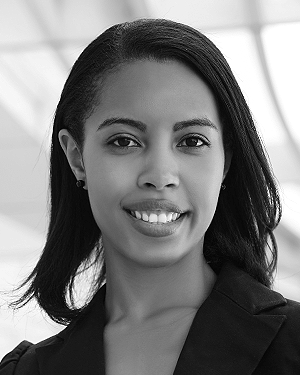
\includegraphics[width=1in,height=1.25in,clip,keepaspectratio]{a1.png}}]{First A. Author} (M'76--SM'81--F'87) and all authors may include 
% biographies. Biographies are often not included in conference-related
% papers. This author became a Member (M) of IEEE in 1976, a Senior
% Member (SM) in 1981, and a Fellow (F) in 1987. The first paragraph may
% contain a place and/or date of birth (list place, then date). Next,
% the author's educational background is listed. The degrees should be
% listed with type of degree in what field, which institution, city,
% state, and country, and year the degree was earned. The author's major
% field of study should be lower-cased. 

% The second paragraph uses the pronoun of the person (he or she) and not the 
% author's last name. It lists military and work experience, including summer 
% and fellowship jobs. Job titles are capitalized. The current job must have a 
% location; previous positions may be listed 
% without one. Information concerning previous publications may be included. 
% Try not to list more than three books or published articles. The format for 
% listing publishers of a book within the biography is: title of book 
% (publisher name, year) similar to a reference. Current and previous research 
% interests end the paragraph. The third paragraph begins with the author's 
% title and last name (e.g., Dr.\ Smith, Prof.\ Jones, Mr.\ Kajor, Ms.\ Hunter). 
% List any memberships in professional societies other than the IEEE. Finally, 
% list any awards and work for IEEE committees and publications. If a 
% photograph is provided, it should be of good quality, and 
% professional-looking. Following are two examples of an author's biography.
% \end{IEEEbiography}

% \begin{IEEEbiography}[{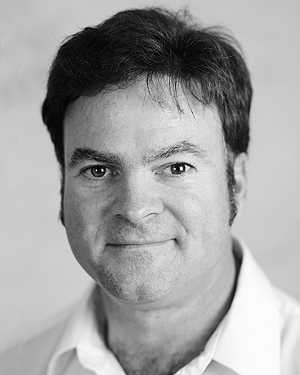
\includegraphics[width=1in,height=1.25in,clip,keepaspectratio]{a2.png}}]{Second B. Author} was born in Greenwich Village, New York, NY, USA in 
% 1977. He received the B.S. and M.S. degrees in aerospace engineering from 
% the University of Virginia, Charlottesville, in 2001 and the Ph.D. degree in 
% mechanical engineering from Drexel University, Philadelphia, PA, in 2008.

% From 2001 to 2004, he was a Research Assistant with the Princeton Plasma 
% Physics Laboratory. Since 2009, he has been an Assistant Professor with the 
% Mechanical Engineering Department, Texas A{\&}M University, College Station. 
% He is the author of three books, more than 150 articles, and more than 70 
% inventions. His research interests include high-pressure and high-density 
% nonthermal plasma discharge processes and applications, microscale plasma 
% discharges, discharges in liquids, spectroscopic diagnostics, plasma 
% propulsion, and innovation plasma applications. He is an Associate Editor of 
% the journal \emph{Earth, Moon, Planets}, and holds two patents. 

% Dr. Author was a recipient of the International Association of Geomagnetism 
% and Aeronomy Young Scientist Award for Excellence in 2008, and the IEEE 
% Electromagnetic Compatibility Society Best Symposium Paper Award in 2011. 
% \end{IEEEbiography}

% \begin{IEEEbiography}[{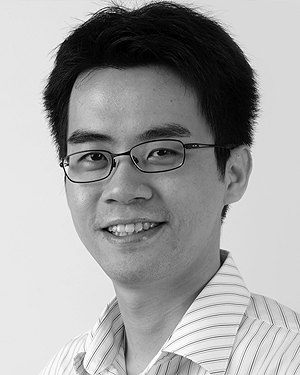
\includegraphics[width=1in,height=1.25in,clip,keepaspectratio]{a3.png}}]{Third C. Author, Jr.} (M'87) received the B.S. degree in mechanical 
% engineering from National Chung Cheng University, Chiayi, Taiwan, in 2004 
% and the M.S. degree in mechanical engineering from National Tsing Hua 
% University, Hsinchu, Taiwan, in 2006. He is currently pursuing the Ph.D. 
% degree in mechanical engineering at Texas A{\&}M University, College 
% Station, TX, USA.

% From 2008 to 2009, he was a Research Assistant with the Institute of 
% Physics, Academia Sinica, Tapei, Taiwan. His research interest includes the 
% development of surface processing and biological/medical treatment 
% techniques using nonthermal atmospheric pressure plasmas, fundamental study 
% of plasma sources, and fabrication of micro- or nanostructured surfaces. 

% Mr. Author's awards and honors include the Frew Fellowship (Australian 
% Academy of Science), the I. I. Rabi Prize (APS), the European Frequency and 
% Time Forum Award, the Carl Zeiss Research Award, the William F. Meggers 
% Award and the Adolph Lomb Medal (OSA).
% \end{IEEEbiography}

\EOD

\end{document}
